\chapter{Experimental Setup}
Over the past 30 years, PVES has become a well-established and powerful experimental technique in atomic, nuclear, and particle physics. Its success can be traced back to Lee and Yang's prediction of parity violation in beta decay in 1956, followed by Wu's experimental proof in 1957. Shortly thereafter, Zel'dovich predicted the existence of parity-violating weak neutral current in 1959 \cite{Zeldovich}, proposing to measure it in electron-proton scattering. However, it took about 20 years for the PV asymmetry to be experimentally observed in electron scattering experiments.

In 1978, C.Y. Prescott et al. conducted the E122 experiment at SLAC, measuring the PV asymmetry in the inelastic scattering of longitudinally polarized electrons from an unpolarized deuterium target \cite{PRESCOTT1978347}. With this successful demonstration, more efforts were made to improve this experimental technique, which matured and flourished at the turn of the last century. Numerous experiments were conducted to investigate the contribution of strange sea quarks to nucleons' electromagnetic form factors (SAMPLE, G0, HAPPEX, and A4) and to test the electroweak sector of the Standard Model (SB) at low-energy scales (E158, PVDIS, Qweak).

It was the PREX-I experiment that first proposed the application of PVES to probe the structure of nuclei, followed by PREX-II and CREX. Future programs such as M\/oller, SoLID, and MESA experiments will continue to develop PVES and enhance its precision.
% First PVES experiment at JLab -- HAPPEX: Hall A Proton Parity EXperiment (E91-010)
% PREX-I is the first EW observation that there is a neutron skin around a heavy nucleus -- https://indico.ihep.ac.cn/event/8987/contributions/105838/attachments/56820/65550/PREXCREX_jlzhang.pdf

\begin{figure}[!h]
    \centering
    \includegraphics[width=0.5\linewidth]{PVES}
    \caption[Evolution of PVES experiments.]
    { The evolution of PVES experiments is depicted by solid lines, which represent the relative precision achieved. Generation I experiments, including E122 (1978) \cite{PRESCOTT1978347}, MIT-12C (1989) \cite{PhysRevLett.65.694}, and Mainz-Be (1990) \cite{HEIL19891}, laid the foundation for PVES research. Generation II experiments focused on exploring strange form factors (FFs) in nucleons and involved collaborations such as SAMPLE \cite{SAMPLE} at the MIT-Bates accelerator, G0 \cite{G0} and HAPPEX \cite{HAPPEX} at JLab, and A4 \cite{A4} at the Maizer Mikrotron (MAMI) accelerator. Generation III experiments, including E158 at SLAC \cite{PhysRevLett.95.081601}, Qweak \cite{PhysRevLett.111.141803}, and PVDIS \cite{PhysRevLett.111.082501}, focused on testing the SM at low energy and measuring the neutron skin thickness of nuclei. Additionally, the PREX-I/II and CREX experiments were conducted to probe the structure of nuclei. The planned Generation IV experiments, namely the SoLID program \cite{SoLID} and the MOLLER experiment \cite{Moller-project} at JLab, and the P2 experiment at the future Mainz Energy-recovery Superconducting Accelerator (MESA) \cite{MESA-P2}, aim to further test the SM and explore the nucleon structure with even higher precision. It's worth noting that MESA-12C refers to the same experiment as MESA-P2 but with a different target, namely \Carbon.
    }
\end{figure}
% precision of PREX-I does not allow to exclude many models, that's why people
% proposed PREX-II.

The idea behind PVES experiments is straightforward: scatter longitudinally polarized electrons off an unpolarized target (such as H, D, He, C, Ca, Pb, etc.) and measure the number of scattered electrons ($N$). Then, reverse the beam helicity and repeat the measurement. The PV asymmetry between different helicities can be calculated as follows:
\begin{equation}
    \CA_{PV} = \frac{N^+/I^+ - N^-/I^-}{N^+/I^+ + N^-/I^-}
\end{equation}
where $I$ is the beam current, and the superscript denotes the beam helicity. 
The procedure described above should be repeated millions of times to obtain a statistically precise result, as the asymmetry being measured is typically extremely small.

% low frequency noise and high frequency noise
% high energy ==> short wavelength: 1 fm⁻¹ ~ 200 MeV
Attention to detail is crucial in PVES experiments. Typically, two essential conditions are required: a high-energy polarized electron beam and rapid flipping of the beam polarization. Interestingly, both requirements share a common dependency: the need for an intense source of polarized electrons with a swift response. It took several decades to develop such an electron source.
At present, the electron source at JLab has achieved a polarization of approximately 90\%. Ongoing efforts are being made to further improve the polarization.

The fast flipping requirement in PVES experiments arises from the need to minimize various sources of noise. When measuring such a minute quantity, it is crucial to maintain consistent experimental conditions across different helicity states. One effective and practical method to meet this requirement is through fast helicity flipping, typically in the range of $10^2 - 10^3$~Hz. By increasing the speed of helicity reversal, random noise in beam conditions, target density, and other experimental apparatus is reduced, thereby minimizing the introduction of false asymmetry. % It is worth noting that this fast flipping requirement sets PVES experiments apart from the capabilities of storage ring accelerators, as meeting such stringent demands is challenging in that context.

While the fast reversal of electron helicity helps in PVES experiments, significant efforts are still required to minimize beam fluctuations. This involves achieving a ``parity-quality beam" (PQB) by carefully controlling and reducing beam fluctuations to the greatest extent possible. Systematic uncertainties arising from the source (injector) and accelerator are managed through the slow reversal of the beam helicity.

In terms of the target's response to electron bombardment, a high-speed raster scanning technique, typically in the range of kHz, is employed to minimize uncertainties associated with target deformities. This rapid scanning helps ensure a more uniform electron beam distribution on the target surface.

Regarding the detection of scattered electrons, instead of counting individual electrons, the electron flux is typically measured due to the high scattering rates in such experiments, which can reach values on the order of MHz per microampere (MHz/$\mu$A). This approach allows for efficient and accurate detection given the high rate of electron scattering.

The two sister experiments were conducted in Hall A at JLab. The CEBAF accelerator \cite{10.1146/annurev.nucl.51.101701.132327} 
at JLab is one of the few facilities worldwide that can carry out PVES experiments
(other facilities capable of conducting PVES experiments include MIMA and its successor MESA, 
the Facility for Antiproton and Ion Research (FAIR) and the Facility for Rare Isotope Beams (FRIB)). 
It delivered excellent polarized electron beams with helicity correlated difference at 
a sub-nanometer level to Hall A. Together with dedicated apparatus in Hall A, such
as polarimeters, a target chamber, high resolution spectrometer (HRS) and other equipment \cite{ALCORN2004294},
we were able to measure the extremely small PV asymmetry with remarkable precision.

% table of beam parameters
\begin{table}[h]
    \centering
    \begin{tabular}{l | c c }
	\hline
	&   PREX-II & CREX  \\
	\hline
	Target	& \Pb	& \Ca	\\
	Target Thickness (mm)	& 0.2554 + 0.5520 + 0.2566\tablefootnote{\Pb target composes of 3 foils: upstream Diamond + \Pb + downstream Diamond}    & 6	\\
	Target Density (g/cm${}^3$)   & 11.38 & 1.855	\\
	Number of Target & 10 & 1 + 1\tablefootnote{Only 1 was prepared for the experiment. After the target accident, a new one was prepared.}	\\ 
	Number of Used Target & 6 & 2	\\
	\hline
	Beam Energy (GeV) & 0.953 & 2.18  \\
	Beam Current ($\mu$A)	& 50-85	& 100-150   \\
	Average Beam Polarization (\%) & 89.7   & 87.1   \\
	% Beam Bunch Rate (MHz)	& 499	& 499 \\
	% Electrons/Bunch	($\times 10^6$)	& 1.75	& 3.76	\\  
	Helicity Flip Rate (Hz) & 120/240   & 120   \\
	Power on the Target	& $\sim100$ W\texttt{@}70~$\mu$A  & $\sim350$ W\texttt{@}150~$\mu$A \\
	\hline
	Scattering Angle ($\deg$)   & 4.7	& 4.51 \\
	$Q^2$ ($\mathrm{GeV}^2$)	& 0.00616   & 0.0297	\\
	Scattering Rate (MHz/$\mu$A/arm)   & $\sim 30$\tablefootnote{This rate does not include the contribution from the diamond foils}   & $\sim0.2$ \\
	% Scattering Rate (1/bunch/arm)   & $\sim 4.5$   & $\sim 0.05$ \\
	Cross section (mbarn)    & 3930.6	& 5.3   \\
	Acceptance (msr)    &	0.0037 & 0.0037  \\
	\hline
	Collected Charge (C)	& 114	& 412	\\
	\hline
	Predicted $\CA_{\text{PV}}$ (ppm)	& 0.6   & 2 \\
	Proposed Precision  &	3\%   & 2.4\% \\
	Error on $R_n$ (fm)	& 0.05	& 0.02	\\
	\hline
    \end{tabular}
    \caption{Summary of experimental design and setup for PREX-II and CREX.}
    \label{tab:parameters}
% crex rate: https://logbooks.jlab.org/entry/3748863
\end{table}

%%%%%%%%%%%%%%%%%%%%%%%%%%%%%%%%%%%%%%%%%%%%%%%%%%%%%%%%%%%%%%%%%%%%%%%%
\section{Beam Parameters}
PREX-II and CREX are follow-up experiments to PREX-I, which also ran at JLab in 2010. 
With quite good control over systematic uncertainties, but unfortunately, 
many technical challenges were encountered during the experiment, PREX-I's result was
statistics-limited, resulting in an achieved precision of 10\% \cite{PhysRevLett.108.112502}:
$$ \CA_{\text{Pb}} = 656 \pm 60 \ (\text{stat}) \pm 14 \ (\text{syst}) \ \text{parts-per-billion (ppb)} $$
Based on the experience and lessons learned from PREX-I, 
PREX-II and CREX have been designed with more robustness and well-established methodologies to achieve high-precision measurements.

A notable feature of these experiments is the redundancy design implemented for critical components. This includes two independent slow helicity reversal systems to control systematic uncertainties, two polarimeters for accurate polarization measurement, multiple beam position monitors (BPMs) and beam current monitors (BCMs) for precise monitoring of beam parameters, multiple \Pb targets, and finally, two high-resolution spectrometers to detect the scattered electrons. These redundant designs enhance the reliability and quality of the experiments.

%%%%%%%%%%%%%%%%%%%%%%%%%%%%%%%%%%%%%%%%%%%%%%%%
\subsection{Uncertainty Budget}
The goal of PREX-II is to achieve a precision of 1\% in the measurement of the 
neutron radius of \Pb, as proposed by PREX-I. This requires improving the 
precision of the PV asymmetry measurement to better than 3\% \cite{PhysRevLett.106.252501}. 

Similarly, CREX aims to reach a precision of $0.02$~fm ($\sim 0.6\%$) in the
determination of the neutron radius of \Ca.
This precise measurement will serve as a crucial benchmark for testing various microscopic models \cite{crex_proposal}. Achieving this level of precision corresponds to a total uncertainty of 2.4\% in the PV asymmetry measurement.

% page 7 in https://prex.jlab.org/DocDB/0000/000065/001/kutz_fom.pdf
As mentioned above, PREX-I has demonstrated a remarkable level of control over 
systematic uncertainties at 2.1\%, so will the PREX-II and CREX. 
The main concern for both experiments is to collect as much scattered 
electrons as possible to reduce statistical uncertainty, which is inversely 
proportional to $\sqrt{N}$, with $N$ being the total number of scattered electrons.
\begin{equation}
    \frac{\delta \CA}{\CA} = \sqrt{\sigma^2_{\text{stat}} + \sigma^2_{\text{sys}}}	
    \qquad 
    \sigma_{\text{stat}} = \frac{\sigma_{\text{det}}}{\CP\sqrt{N}}
\end{equation}
where $\sigma_{\text{det}}$ is the detector uncertainty and $\CP$ refers to the beam polarization.

\begin{table}[!h]
    \centering
    % page 19 in https://www.jlab.org/intralab/calendar/phys_seminar/2019/JLabtalk_20190206mod_Palatchi.pdf
    % Jinlon's slide says a 2% statistical uncertainty for CREX, while Caryn's slide says 4%
    % Paul's slide says 2.4%, maybe the total uncertainty
    \begin{tabular}{c| c c c}
	\hline
	Experiment  & PREX-I (\%)   & PREX-II (\%)	& CREX (\%)	\\
	\hline
	Charge Normalization	& 0.2	& 0.1	& 0.1	\\
	Beam Asymmetry		& 1.1	& 1.1	& 0.3	\\
	Detector Non-Linearity	& 1.2	& 1.0	& 0.3	\\
	Transverse Asymmetry	& 0.2	& 0.2	& 0.1	\\
	Polarization		& 1.3	& 1.1	& 0.8	\\
	Target Contamination	& 0.4	& 0.4	& 0.2	\\
	Inelastic Scattering	& $<0.1\%$  & $<0.1$    & 0.2   \\
	Effective $Q^2$		& 0.5	& 0.4	& 0.8	\\
	\hline
	Total Systematic	& 2.1	& 2	& 1.2	\\
	Statistical		& 9.1	& 2.2	& 2.1	\\
	\hline
	Total			& 9.2	& 3	& 2.4	\\
	\hline
    \end{tabular}
    \caption{Proposed budget for systematic and statistical uncertainties in both experiments 
    \cite{prex-II_proposal, crex_proposal}
    }
\end{table}


%%%%%%%%%%%%%%%%%%%%%%%%%%%%%%%%%%%%%%%%%%%%%%%%
\subsection{Figure Of Merits (FOM)}
The choice of beam energy and scattering angle involves a trade-off between various
factors. The PV asymmetry prefers higher beam energies and a larger scattering angles.
However, the scattering rate decreases significantly with increasing beam energy and scattering angle.
On the other hand, $Q^2$ favors lower beam energies and smaller scattering angles. 
Additionally, calculations demonstrate that the sensitivity of PV asymmetry to the neutron radius oscillates as a function of beam energy.
All these considerations are incorporated into the FOM, which is defined as:
\begin{equation}
    \text{FOM} = R \times \CA^2 \times \epsilon^2
\end{equation}
where R is the scattering rate, $\CA$ the PV asymmetry and $\epsilon$ 
the sensitivity of $\CA$ with respect to $R_n$. It is worth noting that the FOMs used in
most PVES experiments typically consider only R and $\CA^2$. 
The inclusion of $\epsilon$ in our FOM helps to enhance the precision of the $R_n$ measurement.

%%%%%%%%%%%%%%%%%%%%%%%%
% from materials/rate_estimation.pdf
\subsubsection{Rate}
For a data set of N independent events sampled from a normal distribution 
$X\sim N(x_0, \sigma_0)$, the statistical uncertainty on the measured mean value
is:
$$ \text{var}(\bar{x} = \frac{1}{n}\sum x_i) = \frac{1}{n^2}\text{var}(x_i) = \frac{\sigma_0^2}{n} 
\quad \Longrightarrow \sigma(\bar{x}) = \frac{\sigma_0}{\sqrt{n}} $$

Assuming one wants to measure a $1$~ppm asymmetry with a statistical uncertainty of 1\%,
\begin{equation}
    \frac{\sigma_\CA}{\CA} = \frac{1}{\CA}\frac{\sigma_{det}}{\sqrt{2N}} 
    \approx \frac{1}{\CA\sqrt{2N}} = 1\% \quad 
    \Longrightarrow N = 5 \times 10^{15} 
    \label{eq:statistical_error}
\end{equation}
a factor of 2 is included because there are two HRS arms.
One needs to count $\sim10^{15}$ scattered electrons. Given a counting rate of 1~MHz, 
it will take $\frac{5\times 10^{15}}{1\ \mathrm{MHz}} = 5\times 10^{9}\ \mathrm{s} \approx 160$~years,
a completely unacceptable time scale. As a solution, the integrated flux technique is
adopted for a higher scattering rate, which is:
\begin{equation}
    \frac{dR(\theta)}{d\Omega} = \frac{d\sigma}{d\Omega}\ I\ t\ \frac{\rho}{A} \times N_A   
\end{equation}
\begin{itemize}
    \item $\frac{d\sigma}{d\Omega}$ is the fractional cross section in the unit of $\mathrm{cm}^2$/str.
    \item $I$ is the beam current in the unit of electrons/s.
    \item $t$ is the target thickness in the unit of cm.
    \item $\rho$ is the target density in the unit of g/cm${}^3$.
    \item $A$ is the atomic number.
    \item $N_A = 6.022\times 10^{23}$ is the Avogadro constant.
\end{itemize}

The differential cross sections are calculated to be 3930.6~mbarn and 5.3~mbarn 
for \Pb and \Ca, respectively, at their corresponding kinematics. 
Other parameters can be checked out in Table~\ref{tab:parameters}.

The total rate will be the integration over the acceptance:
\begin{equation}
    R = \int \frac{dR(\theta)}{d\Omega} d\Omega = \frac{dR}{d\Omega} d\Omega
\end{equation}
PREX-II and CREX have an acceptance defined by the septum magnet and the Q1 collimator 
(see discussions below), which is $d\Omega = 0.0037$~str.

\begin{comment}
Finally, we should also consider the radiative correction due to emission of virtual
and real soft photons (Bremsstrahlung radiation), and hard photons by vacuum polarization,
this correction is formulated as:
\begin{equation}
    \eta = \left(\frac{\Delta}{E} \right)^{bt}
\end{equation}
which is evaluated to be: $\eta \sim 0.5$.
\end{comment}

As shown in Fig.~\ref{fig:scattering_rate}, the scattering rate decreases 
rapidly with increasing beam energy and scattering angle for both \Pb and \Ca, 
Therefore, in order to achieve a high scattering rate, it is preferable to use 
a low beam energy and a small scattering angle (or equivalently, a small momentum transfer $\vec{q}$).
\begin{figure}[!h]
    \includegraphics[width=0.5\linewidth]{Pb208_rate}
    \includegraphics[width=0.5\linewidth]{Ca48_rate}
    \caption[Scattering rate]
    {Scattering rate versus the beam energy and the scattering angle for \Pb and \Ca,
    the other parameters (energy in the scattering angle plot and vice versa) 
    are fixed to their design values.}
    \label{fig:scattering_rate}
\end{figure}

%%%%%%%%%%%%%%%%%%%%%%%%
\subsubsection{Asymmetry and Sensitivity}
As shown in Eq.~\ref{eq:statistical_error}, the size of the asymmetry plays a crucial role,
a 2 times larger asymmetry allows for a reduction of the run time to one quarter,
a significant savings in beam time. Therefore, it is important to choose a kinematic region where
the asymmetry is large. Furthermore, the sensitivity of the asymmetry to the neutron radius ($\epsilon$) 
is also important. Since our ultimate goal is to extract the neutron radius
from the PV asymmetry, a higher sensitivity leads to a more precise determination
of the neutron radius. The sensitivity is calculated
as the relative change of $\CA$ with 1\% change in the neutron radius.
\begin{equation}
    \epsilon = \frac{\delta \CA/\CA}{\delta R/R} = \frac{|\CA_{stretched} - \CA|/\CA}{1\%}
\end{equation}
Though asymmetry is what will be measured, it is possible to estimate its value based
on some theoretical models, as is calculated in \cite{PhysRevC.57.3430}.
\begin{figure}[!h]
    \includegraphics[width=0.5\linewidth]{Pb208_asym}
    \includegraphics[width=0.5\linewidth]{Pb208_sen}
    \caption[Asymmetry and sensitivity for \Pb]
    {Asymmetry and sensitivity plots for \Pb. The asymmetry increases along 
    the beam energy and oscillates upward along the scattering angle. 
    Similar trends can be observed in the sensitivity plot.
    The sensitivity plot is calculated with 1\% change in the neutron radius and the y-axis
    represent the absolute value.
    At a beam energy of 950~MeV, a local maximum is observed around $theta \sim 6^\circ$.
    }
\end{figure}
\begin{figure}[!h]
    \includegraphics[width=0.5\linewidth]{Ca48_asym}
    \includegraphics[width=0.5\linewidth]{Ca48_sen}
    \caption[Asymmetry and sensitivity for \Ca]
    {Asymmetry and sensitivity plots for \Ca, the asymmetry maximizes
    around 2500~MeV with $\theta = 4^\circ$ and there is a local maximum 
    about $4.5^\circ$ at a beam energy of 2200~MeV. As for the sensitivity, it increases
    monotonously along the beam energy and comes to a regional maximum around $5^\circ$
    with $E$ = 2200~MeV.
    }
    \label{fig:ca48_asym_sen}
\end{figure}

Based on the theoretical result, we can optimize the kinematics for both nuclei 
(consider only the statistical uncertainty here):
\begin{equation}
    \frac{\delta R}{R} = \frac{\delta \CA}{\CA} \frac{1}{\epsilon} 
	= \frac{\sigma_{det}}{\CP} \frac{1}{\sqrt{N} \CA \epsilon}
\end{equation}
To minimize $\delta R/R$, it is equivalent to maximize 
\begin{equation}
    \text{FOM} = N\times \CA^2 \times \epsilon^2
\end{equation}
\begin{figure}
    \includegraphics[width=0.5\linewidth]{Pb208_fom}
    \includegraphics[width=0.5\linewidth]{Ca48_fom}
    \caption[FOM]{For both nuclei, FOM supports a small scattering angle. As for the beam energy,
    FOM maximizes around 950 (2200)~MeV for \Pb (\Ca).}
\end{figure}

Given practical constraints on how low an angle ($4^\circ$) we can reach with 
septum magnets, the beam energy and the scattering angle were chosen to be 950 (2200)~MeV
and 5 (4)~degree for \Pb (\Ca). The beam energy for CREX is exactly a natural 1-pass (1-turn) beam
energy in CEBAF in the 12~GeV era.
\begin{comment}
For PREX-II: average sensitivity reduced by 5\% due to ${}^{12}C$ contamination
For CREX: average sensitivity reduced by 10\% due to ${}^{40}Ca$ contamination

% \subsubsection{Factor of 1.06}
While a quartz Cherenkov detector is valued for radiation hardness and insensitivity to soft backgrounds, there is a particular challenge for few GeV electrons. In this energy range, shower fluctuations in a thick or radiated detector significantly degrade energy resolution, while photon statistics degrade the energy resolution for a thin detector. The energy resolution $\Delta E$ at nominal electron energy E increases the statistical error that one would have with infinite resolution $\sigma_0$ to obtain the total statistical error:
$$ \sigma = \sigma_0\sqrt{1+\left(\frac{\Delta E}{E}\right)^2}$$
    
Based on experience in the PREX experiment, we expect a reduction of statistical precision of a factor of 1.06 due to detector resolution.
\end{comment}

%%%%%%%%%%%%%%%%%%%%%%%%%%%%%%%%%%%%%%%%%%%%%%%%
\subsection{Helicity Flip Frequency}
The main consideration for the choice of the 120~Hz (240~Hz) flip frequency 
was to effectively cancel out the 60 Hz power line noise.

Depending on the desired precision, there are a few methods to mitigate or eliminate this low frequency noise:
\begin{enumerate}
    \item Set the flip frequency to a very high value, say 1~kHz, then
	the change of fluctuations caused by this low frequency noise becomes negligible
	between two nearby helicity windows and canceled in the asymmetry calculation. 
	This method can eliminate many low frequency noises and was adopted in the Qweak experiment.
    \item Integrate over this 60~Hz noise within a helicity window. This integration
	is performed at a frequency of $f = \frac{60}{n}\ \mathrm{Hz}$, where $n$
	is an integer (1, 2, $\cdots$) representing the helicity window number. 
	This way no 60~Hz line noise will be recorded in the final data at all.
    \item Select a flip frequency of $f = n \times 60 \ \mathrm{Hz}$ where $n$
	is an integer. A helicity pattern is then used to cancel the 60~Hz noise. 
	For example, if $f = 120$~Hz, then every $f/30 = 4$ continuous helicity windows form a 
	helicity pattern, asymmetry will be calculated based on these helicity patterns. 
	This was used in PREX-II/CREX.
\end{enumerate}

In terms of canceling the 60~Hz line noise, the second method works best as 
it completely removes the line noise. The other two methods also cancel the noise
in their asymmetry calculation, but result in a broadening of the asymmetry width. 
However, when considering other low frequency noises, the frequency used in 
the second method may not be high enough to cancel them effectively.

The first method is the best for removing low frequency noises, but it has the drawback of a fixed settle time ($T_{\text{settle}}$) required to stabilize a helicity state. With higher frequencies, the stable time window ($T_{\text{stable}}$) during which scattered electrons are integrated becomes shorter, leading to longer run times.

As a compromise, the third method was chosen for PREX-II/CREX. It provides a reasonable balance between canceling low frequency noises and maintaining an acceptable settle time and run time.

%%%%%%%%%%%%%%%%%%%%%%%%%%%%%%%%%%%%%%%%%%%%%%%%%%%%%%%%%%%%%%%%%%%%%%%%
\section{Continuous Electron Beam Accelerator Facility (CEBAF)}
\begin{figure}[!h]
    \begin{subfigure}[b]{0.59\textwidth}
    \begin{tikzpicture}
	\begin{scope}
	    \node[anchor=south west, inner sep=0] (image) at (0, 0)
	    { \includegraphics[width=\linewidth]{jlab.jpg} };
	    \begin{scope}[x={(image.south east)}, y={(image.north west)}]
		\node [red] at (0.415, 0.355) {\textbf{A}};
		\node [red] at (0.610, 0.355) {\textbf{B}};
		\node [red] at (0.780, 0.355) {\textbf{C}};
	    \end{scope}
	\end{scope}
    \end{tikzpicture}
    \end{subfigure}
    \begin{subfigure}[b]{0.5\textwidth}
	\includegraphics[width=0.9\linewidth]{tunnel_construction}
	\includegraphics[width=0.9\linewidth]{hall_construction}
    \end{subfigure}

    \caption[JLab aerial view]
    {Aerial view of JLab accelerator site. The yellow line indicates the position
    of the CEBAF accelerator, while the three experimental halls are labeled as A/B/C 
    (Hall D is situated at the top left corner, after the exit of the north LINAC).
    The accelerator tunnel is located 30~feet ($\sim 9$~m) underground and has 
    a height of 10~feet ($\sim 3$~m). It has a circumference of about 7/8~mile (1.4~km). 
    There are two superconducting LINACs depicted as red lines, each of 1/4~mile (400~m). 
    The pink section on the mid-left represents the location of the injector. 
    The two plots on the right show the ongoing construction of the tunnel and 
    experimental halls.}
\end{figure}

\begin{figure}[!h]
    \includegraphics[width=0.9\linewidth]{cebaf.png}
    \caption[CEBAF]
    {Schematic plot of CEBAF. The circular plate with three slits is the beam chopper,
    which does not have a slit for Hall D. As a result, Hall D beams must follow 
    the electron beams of other halls. During acceleration, low-energy beams are kicked into 
    higher arcs, while high-energy beams pass through lower arcs. The magnetic
    field increases from the higher arcs to the lower arcs to ensure that electron trajectories
    have the same radii.}
    \label{fig:cebaf}
\end{figure}
CEBAF is capable of delivering multi-GeV continuous wave (cw) electron beams with
varying energies and intensities to four experimental halls simultaneously.
With the 12~GeV upgrade, the injector energy has been increased from 67.5~MeV to 
123~MeV. The north and south 1497~MHz linear accelerators (LINACs) each consist of 25 
superconducting radial frequency (SRF) cryomodules, allowing for electron acceleration
at a peak rate of $1.1 \times 2 = 2.2$~GeV/turn. The LINACs are connected 
by 11 arcs of magnets, allowing Hall A, B and C to receive cw beams with energies 
of up to $2.2 \times 5 = 11$~GeV. Hall D, with an additional half circle,
can receive beams with energies up to 12~GeV. This design enables different nuclear 
experiments to be conducted in separate halls without interfering each other,
in theory.

As shown in Fig.~\ref{fig:cebaf}, laser pulse ($\lambda = 780$~nm) from four lasers 
(Hall D laser is not shown in the plot) shoot in the electron gun 
(two electron guns in total) that operates at $-130$~kV to excite electrons. 
These excited electrons interweave with each other, forming a chain of electron bunches, 
Adjacent bunches have a phase difference of $120^\circ$ (Hall D does not have 
its own slit in the beam chopper. Therefore, the electron bunch from hall D 
follows either Hall A or Hall C). The electron chain is initially sent into the 
north LINAC by the injector and accelerated by both LINACs. Once they reach the desired energy,
they are expelled at the exit of the south LINAC and subsequently directed towards 
the experimental halls (A, B and C) for various experiments. 

At CEBAF, the maximum beam current available is 200 $\mu$A. This current limitation was primarily determined by two factors: the available radiofrequency (rf) power and the power deposited on the beam dump. The rf power was limited to 1 MW, which corresponded to the product of the old highest beam energy (5 GeV) and the maximum beam current (200 $\mu$A).

While Hall B and Hall D require only a small amount of cw beams at the nA level, it is actually Hall A and Hall C that consume the majority of the electron beams. Both halls can receive cw beams ranging from a few tenths to over one hundred $\mu$A. 

While all four halls at JLab are dedicated to the study of nuclear structure, they
focus on different aspects. Hall A concentrates on form factors of various nuclei, 
Hall B focuses on generalized parton distributions, Hall C is dedicated to precise
determination of valence quark properties in nuclei, and finally, the newly 
established Hall D explores the origin of confinement through exotic mesons.
\begin{figure}[!h]
    \centering
    \includegraphics[width=0.48\linewidth]{hall_A}
    \includegraphics[width=0.51\linewidth]{hall_A_bird}
    \caption[Hall A]
    {3D and bird view of Hall A \cite{halla_manual}. Originally, the 2 spectrometers
    were called High Resolution Hadron Spectrometer (HRHS) and High Resolution Electron
    Spectrometer (HRES), but they are essentially identical to each other and
    can be used interchangeably.
    So now they are called left arm (LHRS) and right arm HRS (RHRS).
    }
\end{figure}

Since all four halls share the same electron source and accelerator, 
coordination is required to ensure their simultaneous operations. 
In order to maintain the quality of the polarized electron beam, PVES experiments are typically given priority over other experiments when it comes to the electron source. Regarding the LINACs, adjustments are made to accommodate different energy requirements. For instance, if one hall requests a lower energy, such as 1 GeV, the LINAC power will be adjusted accordingly to deliver 1 GeV per turn. However, this adjustment affects the available energy for other halls since the reduced LINAC power is applied to all electron beams. Consequently, careful scheduling is necessary to allocate the appropriate energy levels to each hall based on their specific experimental needs.
%%%%%%%%%%%%%%%%%%%%%%%%%%%%%%%%%%%%%%%%%%%%%%%%%%%%%%%%%%%%%%%%%%%%%%%%
\section{Polarized Electron Beam}
% The key to the success of this experiment was the 1975 discovery of a new method for producing
% polarized electrons made by a group in Colorado, which included E.L. Garwin of SLAC.
% Shortly thereafter, a new source was built for the SLAC linac utilizing the method, thus
% allowing for the 1978 parity violation measurements which were in close agreement with
% those predicted by the GWS model. 

%%%%%%%%%%%%%%%%%%%%%%%%%%%%%%%%%%%%%%%%%%%%%%%%
\subsection{Polarized Electron Source}
PVES experiments are a driving force behind the development of polarized electron sources. 
These sources are essential for generating consistently high-polarization 
electron beams across a wide range of intensities, from nA to A, 
depending on the specific experiment. Additionally, the source should be 
capable of rapid helicity reversal, at a frequency of $\sim 100-1000$~Hz, while 
having minimal impact on other properties of the electron beam.

Currently, the GaAs-based semiconductor photoemission source is % confirmed by Wang Yan
the sole option available on the market as a polarized electron source.
Historically, this kind of electron source was the only one capable of meeting
the high peak current requirements of older accelerators with low duty factors 
and the rapid helicity reversal demands of PVES experiments. 
That is why it is the only player on the market now.
Over the past few decades, pulsed beam has been replaced by continuous beam while
the GaAs-based electron source is inherited and further developed. The polarized electron
source utilized by CEBAF, for instance, can produce electron beams with a polarization exceeding
85\%, much larger than the 37\% polarization achieved during its inauguration at SLAC. \cite{PRESCOTT1978347}

The design was first proposed independently by Garwin, Pierce and Siegmann \cite{GARWIN}
and by Lampel and Weisbuch \cite{LAMPEL1975877}. The idea is straightforward:
by illuminating the semiconductor with circularly polarized laser light of carefully chosen energy
$E_{\text{gap}} < h\nu < E_{\text{gap}} + \Delta$, only electrons in the valance band $P_{3/2}$ are
excited into the conduction band $S_{1/2}$. The selection rule ensures that only
transitions satisfying $\Delta m_j = +1 \ (-1)$ can occur for right (left) circularly
polarized photons, as shown in Fig.~\ref{fig:excitation}.
The transition rates can be calculated easily using Clebsch-Gordan coefficients, % FIXEM reference
and the ratio of these rates is indicated within the circle in the plot.
As a result, the excited electrons become polarized, with different states having different pumping rate.
In this way, a polarized electron beam is produced, with a polarization given by $\CP$ = (3-1)/(3+1) = 50\%,
for both helicities.
\begin{figure}[!h]
    \tikzmath{\yone=1.3; \ytwo=2.5; \ythree=5;} 
    \centering
    \begin{subfigure}[b]{0.49\textwidth}
	\centering
	\begin{tikzpicture}
	    \centering
	    \begin{axis}[axis lines=middle,
		xmin=-1.4, xmax=2.75,
		ymin=0, ymax=7,
		xlabel={\large $k$},
		ylabel={\large$E$},
		xlabel style={below},
		xtick=\empty,
		ytick=\empty,
		x axis line style={draw=none},
		% clip=false,
		]
		\addplot[Violet, line width=3pt, samples=100, domain=-0.7:0.7, name path=A] {-2*x^2 + \yone};
		\addplot[OliveGreen, line width=3pt, samples=100, domain=-0.7:0.7, name path=B] {-2*x^2 + \ytwo};
		\addplot[OliveGreen, line width=3pt, samples=100, domain=-0.7:0.7, name path=B] {-1.2*x^2 + \ytwo};
		\addplot[Blue, line width=3pt, samples=100, domain=-0.7:0.7, name path=B] {2*x^2 + \ythree};
		\draw [/pgfplots/every inner x axis line, draw=black] (0,0) -- (\pgfkeysvalueof{/pgfplots/xmax}, 0); 
		\draw [dashed, draw=black] (0,\yone) -- (\pgfkeysvalueof{/pgfplots/xmax}, \yone);
		\draw [dashed, draw=black] (0,\ytwo) -- (\pgfkeysvalueof{/pgfplots/xmax}, \ytwo);
		\draw [dashed, draw=black] (0,\ythree) -- (\pgfkeysvalueof{/pgfplots/xmax}, \ythree);
		\draw [stealth-stealth, thick] (0.8, \yone) -- (0.8, \ytwo) node [midway, right] {\bm{$\Delta = 0.34\ \mathrm{eV}$}};
		\draw [stealth-stealth, thick] (0.8, \ytwo) -- (0.8, \ythree) node [midway, right] {\bm{$E_{\text{gap}} = 1.42\ \mathrm{eV}$}};
		\node [Violet, below] at (-1, \yone) {\large\bm{$P_{1/2}$}};
		\node [OliveGreen, below] at (-1, \ytwo) {\large\bm{$P_{3/2}$}};
		\node [Blue, above] at (-1, \ythree) {\large\bm{$S_{1/2}$}};
		\node [left, above] at (-0.2, \ytwo) {\large\bm{$E_F$}};
	    \end{axis}
	\end{tikzpicture}
    \end{subfigure}
    \hfill
    \begin{subfigure}[b]{0.49\textwidth}
	\centering
	\begin{tikzpicture}
	    \begin{axis}[axis lines=middle,
		xmin=0, xmax=8,
		ymin=0, ymax=7,
		xlabel={\large $m_j$},
		ylabel={\large$E$},
		xlabel style={below},
		xtick=\empty,
		ytick=\empty,
		]
		\draw [/pgfplots/every inner y axis line, draw=black] (6.5,0) -- (6.5, \pgfkeysvalueof{/pgfplots/ymax}) node [below right] {\large J}; 
		\draw [draw=Violet, line width=2pt] (1.25,\yone) -- (2.25, \yone) node [midway, below, Violet] {\textbf{-1/2}};
		\draw [draw=Violet, line width=2pt] (4.25,\yone) -- (5.25, \yone) node [midway, below, Violet] {\textbf{+1/2}};
		\draw [draw=OliveGreen, line width=2pt] (0.5,\ytwo) -- (1.5, \ytwo) node [midway, below, OliveGreen] {\textbf{-3/2}};
		\draw [draw=OliveGreen, line width=2pt] (2,\ytwo) -- (3, \ytwo) node [midway, below, OliveGreen] {\textbf{-1/2}};
		\draw [draw=OliveGreen, line width=2pt] (3.5,\ytwo) -- (4.5, \ytwo) node [midway, below, OliveGreen] {\textbf{+1/2}};
		\draw [draw=OliveGreen, line width=2pt] (5,\ytwo) -- (6, \ytwo) node [midway, below, OliveGreen] {\textbf{+3/2}};
		\draw [draw=Blue, line width=2pt] (2,\ythree) -- (3, \ythree) node [midway, above, Blue] {\textbf{-1/2}};
		\draw [draw=Blue, line width=2pt] (3.5,\ythree) -- (4.5, \ythree) node [midway, above, Blue] {\textbf{+1/2}};
		\node [Violet, right] at (6.7, \yone-0.1) {\large\bm{$P_{1/2}$}};
		\node [OliveGreen, right] at (6.7, \ytwo-0.1) {\large\bm{$P_{3/2}$}};
		\node [Blue, right] at (6.7, \ythree-0.1) {\large\bm{$S_{1/2}$}};

		\draw [-stealth, Red, line width=2pt] (1, \ytwo) -- (2.5, \ythree) node [midway, circle, fill=CornflowerBlue, text=Black] {\textbf{3}};
		\draw [-stealth, Red, line width=2pt] (2.5, \ytwo) -- (4, \ythree);
		\node [above, Red] at (1, \ytwo+0.5) {\bm{$\sigma^+$}};
		\draw [-stealth, YellowOrange, line width=2pt] (4, \ytwo) -- (2.5, \ythree) node [midway, circle, fill=CornflowerBlue, text=Black] {\textbf{1}};
		\draw [-stealth, YellowOrange, line width=2pt] (5.5, \ytwo) -- (4, \ythree) node [midway, circle, fill=CornflowerBlue, text=Black] {\textbf{3}};
		\node [above, YellowOrange] at (5.5, \ytwo+0.5) {\bm{$\sigma^-$}};
	    \end{axis}
	\end{tikzpicture}
    \end{subfigure}
    \caption{Excitation of electrons in the semiconductor. Excited electrons with $J_z =$ +1/2 (-1/2) are right (left)-handed.}
    \label{fig:excitation}
\end{figure}

\begin{figure}[!h]
    \centering
    \begin{subfigure}[b]{0.32\textwidth}
	\tikzmath{\yone=2.5; \ytwo=5; \ythree=9.5;} 
	\centering
	\resizebox{\textwidth}{0.33\textheight}{
	\begin{tikzpicture}
	    \centering
	    \begin{axis}[
		axis lines=middle,
		xmin=-3, xmax=1,
		ymin=0, ymax=10,
		hide axis,
		]
		\draw [dashed] (\pgfkeysvalueof{/pgfplots/xmin}, \yone) -- (0, \yone) node [right] {\bm{$E_F$}};
		\draw [dashed] (\pgfkeysvalueof{/pgfplots/xmin}, \ytwo) -- (0, \ytwo);
		\draw [dashed] (\pgfkeysvalueof{/pgfplots/xmin}, \ythree) -- (0, \ythree);
		\draw [Violet, line width=2pt] (0, 0) -- (0, \ythree) -- (\pgfkeysvalueof{/pgfplots/xmax}/4, \ythree) node [right, Black] {\bm{$E_\infty$}};
		\fill [pattern=north east lines] (\pgfkeysvalueof{/pgfplots/xmin}, \yone)  -- (-1, \yone) arc (90:0:1) -- (0, 0) -- (\pgfkeysvalueof{/pgfplots/xmin}, 0) -- (\pgfkeysvalueof{/pgfplots/xmin}, \yone);
		\draw [Violet, line width=2pt] (\pgfkeysvalueof{/pgfplots/xmin}, \yone)  -- (-1, \yone) arc (90:0:1);
		\draw [Violet, line width=2pt] (\pgfkeysvalueof{/pgfplots/xmin}, \ytwo)  -- (-1, \ytwo) arc (90:0:1);
		\draw [stealth-stealth, thick] (\pgfkeysvalueof{/pgfplots/xmin} + 0.8, \yone) -- (\pgfkeysvalueof{/pgfplots/xmin} + 0.8, \ytwo) node [midway, left] {\bm{$E_{\text{gap}}$}};
		\draw [stealth-stealth, thick, Red] (-0.5, \ytwo) -- (-0.5, \ythree) node [midway, left] {\textbf{PEA = 4.07~eV}};
		\node [Red, above] at (\pgfkeysvalueof{/pgfplots/xmin}/2, 0) {\textbf{GaAs}};
		\node [Red, above right] at (0, 0) {\textbf{Vac}};
		\node [below left, text width=2cm] at (-0.5, \yone) {\textbf{Valance Band}};
		\node [below left, text width=2cm] at (-0.5, \ytwo) {\textbf{Conduction Band}};
	    \end{axis}
	\end{tikzpicture}
	}
	\label{fig:PEA}
    \end{subfigure}
    \hfill
    \begin{subfigure}[b]{0.32\textwidth}
	\tikzmath{\yone=2.5; \ytwo=5; \ythree=9.5;} 
	\centering
	\resizebox{\textwidth}{0.33\textheight}{
	\begin{tikzpicture}
	    \centering
	    \begin{axis}[
		axis lines=middle,
		xmin=-3, xmax=1,
		ymin=0, ymax=10,
		hide axis,
		]
		\draw [dashed] (\pgfkeysvalueof{/pgfplots/xmin}, \yone) -- (0, \yone) node [right] {\bm{$E_F$}};
		\draw [dashed] (\pgfkeysvalueof{/pgfplots/xmin}, \ytwo) -- (0, \ytwo);
		\node at (0, \pgfkeysvalueof{/pgfplots/ymax}) {};
		\draw [OliveGreen, line width=5pt] (-0.07, 0) -- (-0.07, \ytwo);
		\draw [Violet, line width=2pt] (0, 0) -- (0, \ytwo) -- (\pgfkeysvalueof{/pgfplots/xmax}/4, \ytwo) node [right, Black] {\bm{$E_\infty$}};
		\fill [pattern=north east lines] (\pgfkeysvalueof{/pgfplots/xmin}, \yone)  -- (-1, \yone) arc (90:0:1) -- (0, 0) -- (\pgfkeysvalueof{/pgfplots/xmin}, 0) -- (\pgfkeysvalueof{/pgfplots/xmin}, \yone);
		\draw [Violet, line width=2pt] (\pgfkeysvalueof{/pgfplots/xmin}, \yone)  -- (-1, \yone) arc (90:0:1);
		\draw [Violet, line width=2pt] (\pgfkeysvalueof{/pgfplots/xmin}, \ytwo)  -- (-1, \ytwo) arc (90:0:1);
		\node [Red, above] at (\pgfkeysvalueof{/pgfplots/xmin}/2, 0) {\textbf{GaAs}};
		\node [Red, above] at (-0.03, 0) {\textbf{Cs}};
		\node [Red, above right] at (0.1, 0) {\textbf{Vac}};
	    \end{axis}
	\end{tikzpicture}
	}
	\label{fig:ZEA}	% zero EA
    \end{subfigure}
    \hfill
    \begin{subfigure}[b]{0.32\textwidth}
	\tikzmath{\yone=2.5; \ytwo=5; \ythree=4; \surface=0.8;} 
	\centering
	\resizebox{\textwidth}{0.33\textheight}{
	\begin{tikzpicture}
	    \centering
	    \begin{axis}[
		axis lines=middle,
		xmin=-3, xmax=1,
		ymin=0, ymax=10,
		hide axis,
		]
		\draw [dashed] (\pgfkeysvalueof{/pgfplots/xmin}, \yone) -- (0, \yone) node [right] {\bm{$E_F$}};
		\draw [dashed] (\pgfkeysvalueof{/pgfplots/xmin}, \ytwo) -- (0, \ytwo);
		\draw [dashed] (\pgfkeysvalueof{/pgfplots/xmin}, \ythree) -- (0, \ythree);
		\node at (0, \pgfkeysvalueof{/pgfplots/ymax}) {};
		\draw [Violet, line width=2pt] (0, 0) -- (0, \ythree) -- (\pgfkeysvalueof{/pgfplots/xmax}/4, \ythree) node [right, Black] {\bm{$E_\infty$}};
		\fill [pattern=north east lines] (\pgfkeysvalueof{/pgfplots/xmin}, \yone)  -- (-1-\surface, \yone) arc (90:0:1) -- (-\surface, 1.4) arc (180:270:\surface) --  (0, 0) -- (\pgfkeysvalueof{/pgfplots/xmin}, 0) -- (\pgfkeysvalueof{/pgfplots/xmin}, \yone);
		\draw [Violet, line width=2pt] (-\surface, 0) -- (-\surface, \ytwo/2 + \ythree/2) arc (180:270:\surface);
		\draw [Violet, line width=2pt] (-\surface, 1.4) arc (180:270:\surface);
		\draw [Violet, line width=2pt] (\pgfkeysvalueof{/pgfplots/xmin}, \yone)  -- (-1-\surface, \yone) arc (90:0:1);
		\draw [Violet, line width=2pt] (\pgfkeysvalueof{/pgfplots/xmin}, \ytwo)  -- (-1-\surface, \ytwo) arc (90:0:1);
		\node [Red, above] at (\pgfkeysvalueof{/pgfplots/xmin}/2, 0) {\textbf{GaAs}};
		\node [Red, above] at (-0.4, 0) {\bm{$Cs_2O$}};
		\node [Red, above right] at (0.1, 0) {\textbf{Vac}};

		\node (e1) at (\pgfkeysvalueof{/pgfplots/xmin}/5*3, \yone)[circle, fill=CornflowerBlue, text=Black] {\textbf{e}};
		\node (e2) at (\pgfkeysvalueof{/pgfplots/xmin}/5*3, \ytwo)[circle, fill=CornflowerBlue, text=Black] {\textbf{e}};
		\node (e3) at (0.2, \ythree*1.1)[circle, fill=CornflowerBlue, text=Black] {\textbf{e}};
		\draw [-stealth, thick, CornflowerBlue] (e1) -- (e2);
		\draw [-stealth, thick, CornflowerBlue] (e2) -- (e3);
		\draw [stealth-stealth, thick, Red] (-2.2, \ytwo) -- (-2.2, \ythree) node [midway, left] {\textbf{NEA}};
	    \end{axis}
	\end{tikzpicture}
	}
	\label{fig:NEA}
    \end{subfigure}
    \caption[Energy band diagram of GaAs]
    {The energy band diagram of GaAs near its surface. 
    Left: bare p-type GaAs, the large positive electron affinity (PEA) 
    prevents electrons from escaping the surface; 
    Middle: p-type GaAs with a cesiated surface, the electron affinity (EA)
    is 0, but electrons still cannot escape the surface easily; 
    Right: GaAs with a layer of cesium oxide; the electron vacuum energy $E_\infty$ is
    lowered to make a negative EA so that electrons can break free from the surface
    easily. \cite{CARDMAN1992317}}
    \label{fig:electron_affinity}
\end{figure}
The next challenge is to liberate the polarized electrons from the material without 
significantly degenerating the polarization. As illustrated in Fig.~\ref{fig:electron_affinity},
bare GaAs possesses an electron affinity (EA) of 4.07~eV, which hinders the escape 
of any electrons from the surface. To overcome this hurdle, a condition known as negative
electron affinity (NEA) is employed. This involves reducing the energy of the electron in 
the vacuum just outside the surface to a level lower than the conduction band energy. 
This is achieved by applying a layer of cesium oxide on the surface of a pure GaAs semiconductor.

While the NEA technique enables the generation of polarized electron beams, it falls short of achieving the ideal 50\% polarization. Instead, the achieved polarization typically ranges from 25\% to 43\%. This loss in polarization occurs due to spin dilution as electrons diffuse towards the semiconductor surface. To increase polarization, one approach is to reduce the thickness of the GaAs crystal. However, even with the thinnest possible GaAs crystal, a polarization greater than 50\% cannot be achieved. This calls for new strategies and the answer is the strained GaAs \cite{CARDMAN1992317}.

By introducing a strained layer, the degeneracy of the $P_{3/2}$ state in GaAs is split.
Only states with $m_j = \pm 3/2$ will be selectively pumped, leading to a theoretical
maximum polarization of 100\%. In practice, the achieved polarization is lower due to various factors.
In the case of the CEBAF electron source, the real polarization achieved is approximately 88\%.
\begin{figure}[!h]
    \tikzmath{\yone=1.3; \ytwo=2.5; \ythree=5;} 
    \centering
    \begin{subfigure}[b]{0.49\textwidth}
	\centering
	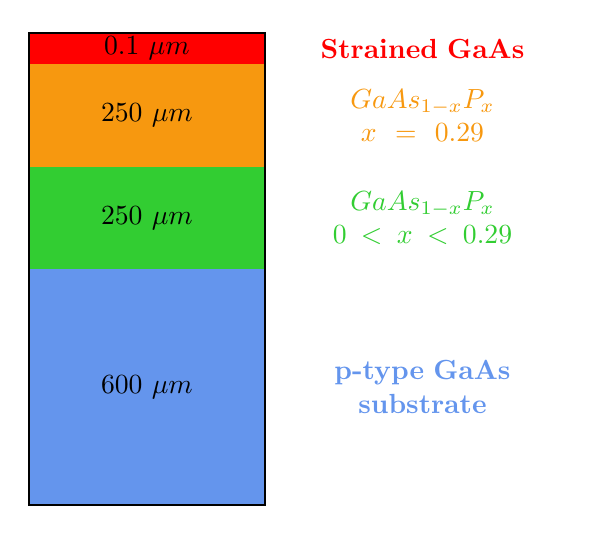
\begin{tikzpicture}
	    \tikzstyle{explain} = [align=center] 
	    \centering
	    \fill [CornflowerBlue] (0, 0) rectangle (3, 3);
	    \node at (3/2, 3/2) {\bm{$600 \ \mu m$}};
	    \node [explain, CornflowerBlue, text width=3.4 cm] at (5, 3/2) {\textbf{p-type GaAs substrate}};
	    \fill [LimeGreen] (0, 3) rectangle (3, 3+1.3);
	    \node at (3/2, 3 + 1.3/2) {\bm{$250 \ \mu m$}};
	    \node [explain, LimeGreen, text width=3.5 cm] at (5, 3+1.3/2) {\bm{$GaAs_{1-x}P_x$} \\ \bm{$0 < x < 0.29$}};
	    \fill [YellowOrange] (0, 3+1.3) rectangle (3, 3+1.3+1.3);
	    \node at (3/2, 3 + 1.3 + 1.3/2) {\bm{$250 \ \mu m$}};
	    \node [explain, YellowOrange, text width=3.5 cm] at (5, 3+1.3+1.3/2) {\bm{$GaAs_{1-x}P_x$} \\ \bm{$x = 0.29$}};
	    \fill [Red] (0, 3+1.3+1.3) rectangle (3, 6);
	    \node at (3/2, 3 + 1.3 + 1.3 + 0.4/2) {\bm{$0.1 \ \mu m$}};
	    \node [explain, Red, text width=3.5 cm] at (5, 3+1.3+1.3+0.4/2) {\textbf{Strained GaAs}};
	    \draw [thick] (0, 0) rectangle (3, 6);
	    \label{fig:excitation-a}
	\end{tikzpicture}
    \end{subfigure}
    \hfill
    \begin{subfigure}[b]{0.49\textwidth}
	\centering
	\begin{tikzpicture}
	    \begin{axis}[axis lines=middle,
		xmin=0, xmax=8,
		ymin=0, ymax=7,
		xlabel={\large $m_j$},
		ylabel={\large$E$},
		xlabel style={above},
		xtick=\empty,
		ytick=\empty,
		]
		\draw [/pgfplots/every inner y axis line, draw=black] (6.5,0) -- (6.5, \pgfkeysvalueof{/pgfplots/ymax}) node [below right] {\large J}; 
		\draw [draw=Violet, line width=2pt] (1.25,\yone) -- (2.25, \yone) node [midway, below, Violet] {\textbf{-1/2}};
		\draw [draw=Violet, line width=2pt] (4.25,\yone) -- (5.25, \yone) node [midway, below, Violet] {\textbf{+1/2}};
		\draw [draw=OliveGreen, line width=2pt] (0.5,\ytwo) -- (1.5, \ytwo) node [midway, below, OliveGreen] {\textbf{-3/2}};
		\draw [draw=OliveGreen, line width=2pt] (2,\ytwo-0.5) -- (3, \ytwo-0.5) node [midway, below, OliveGreen] {\textbf{-1/2}};
		\draw [draw=OliveGreen, line width=2pt] (3.5,\ytwo-0.5) -- (4.5, \ytwo-0.5) node [midway, below, OliveGreen] {\textbf{+1/2}};
		\draw [draw=OliveGreen, line width=2pt] (5,\ytwo) -- (6, \ytwo) node [midway, below, OliveGreen] {\textbf{+3/2}};
		\draw [draw=Blue, line width=2pt] (2,\ythree) -- (3, \ythree) node [midway, above, Blue] {\textbf{-1/2}};
		\draw [draw=Blue, line width=2pt] (3.5,\ythree) -- (4.5, \ythree) node [midway, above, Blue] {\textbf{+1/2}};
		\node [Violet, right] at (6.7, \yone-0.1) {\large\bm{$P_{1/2}$}};
		\node [OliveGreen, right] at (6.7, \ytwo-0.1) {\large\bm{$P_{3/2}$}};
		\node [Blue, right] at (6.7, \ythree-0.1) {\large\bm{$S_{1/2}$}};

		\draw [-stealth, Red, line width=2pt] (1, \ytwo) -- (2.5, \ythree) node [above, midway, sloped] {\bm{$\sigma^+$}};
		\draw [-stealth, YellowOrange, line width=2pt] (5.5, \ytwo) -- (4, \ythree) node [above, midway, sloped] {\bm{$\sigma^-$}};
	    \end{axis}
	\end{tikzpicture}
	\label{fig:excitation-b}
    \end{subfigure}
    \caption{Layout of a strained GaAs electron source and corresponding excitation plot.}
\end{figure}

%%%%%%%%%%%%%%%%%%%%%%%%%%%%%%%%%%%%%%%%%%%%%%%%
\subsection{Polarization Control}
\begin{figure}[!h]
    \includegraphics[width=\linewidth]{injector}
    \caption{The laser system at the CEBAF injector}
    \label{fig:injector}
\end{figure}

\begin{figure}[!h]
    \begin{tikzpicture}
	\tikzstyle{explain} = [align=center] 
	\begin{scope}
	    \node[anchor=south west, inner sep=0] (image) at (0, 0)
	    {\includegraphics[width=\linewidth]{laser_table}};
	    \begin{scope}[x={(image.south east)},y={(image.north west)}]
		\node [blue,ultra thick] at (0.06,0.3) {\textbf{A}};
		\node [blue,ultra thick] at (0.06,0.49) {\textbf{B}};
		\node [blue,ultra thick] at (0.06,0.67) {\textbf{C}};
		\node [blue,ultra thick] at (0.06,0.85) {\textbf{D}};

		\node [blue,ultra thick] at (0.47,0.39) {\textbf{IA}};
		\node [blue,ultra thick] at (0.47,0.56) {\textbf{IA}};
		\node [blue,ultra thick] at (0.5,0.75) {\textbf{IA}};

		\node [red] at (0.75,0.23) {\textbf{IHWP}};
		\node [explain,red] at (0.76,0.33) {\textbf{Pockels } \\ \textbf{Cell}};
		\node [red] at (0.78,0.52) {\textbf{RHWP}};
		\node [explain,red] at (0.88, 0.96) {\textbf{Beamline} \\ \textbf{vacuum} \\ \textbf{window}};
	    \end{scope}
	\end{scope}
    \end{tikzpicture}
    \caption{Schematic plot of the laser table.}
    \label{fig:laser_table}
\end{figure}

%%%%%%%%%%%%%%%%%%%%%%%%%
\subsubsection{Pockels Cell}
To achieve better control over the beam polarization in the production of polarized electron beams, it is necessary to have the ability to quickly flip the polarization while maintaining its stability. Direct manipulation of electrons can be challenging and time-consuming, whereas manipulating photons is comparatively easier. By reversing the circular polarization of the incident laser pulse, the polarization of the electron beam can be flipped. One convenient method to accomplish this is by using a half-wave plate. By inserting or retracting the half-wave plate into/from the optical path, the phase of the laser pulse will be altered by $\pi$, resulting in the reversal of the laser's circular polarization. This simple adjustment provides an effective means of flipping the electron beam polarization.

The drawback of the half-wave plate is that its relatively slow mechanical movement 
is insufficient for the rapid flipping of beam polarization required in PVES experiments.
To address this issue, a component called Pockels cell (PC) is employed.
The PC is a Rubidium Titanyle Phosphate (RTP) crystal that operates based on the Pockels effect. 
The Pockels effect refers to the induction of birefringence in the crystal when subjected to an electric field. The magnitude of the induced birefringence is directly proportional to the strength of the applied electric field. By applying an appropriate high voltage of $\sim$ 1.5~kV, % from Caryn's thesis
the PC acts as a quarter-wave plate. This means that when a linearly polarized laser beam passes through the PC, the electric field components along the fast and slow axes of the crystal, denoted as $E_x$ and $E_y$ respectively, acquire a phase difference of $\pm \frac{\pi}/2$ depending on the polarity of the applied electric field. Consequently, the PC converts the linearly polarized laser beam into a circularly polarized one. Reversing the electric field polarity in the PC allows for the reversal of the laser beam's polarization. This transition in the PC can be accomplished swiftly, reaching frequency of up to 1~kHz, with a dead time of about 60~$\mu$s. 
% Moller will go up to 2 kHz, with 10 \mu s settle time

\subsubsection{Polarization Induced Transport Asymmetry (PITA, or Phase Induced Transmission Asymmetry) \cite{Caryn2019}}
The above discussion presented an ideal scenario where the PC functions as a precise quarter-wave
plate, and all other optical components operate flawlessly. However, in reality, there are always deviations from perfect circular polarization, leading to systematic effects on beam position, spot size, and intensity.
These deviations, when correlated with polarization, can introduce a false asymmetry in our PV asymmetry measurement. This phenomenon is known as the PITA effect. The PITA effect constitutes the dominant component of the helicity-correlated beam asymmetry (HCBA) and represents the largest false asymmetry in our measurement.

\begin{figure}[!h]
    \centering
    \includegraphics[width=0.5\linewidth]{PC_phase_shift}
    \caption{Phase shift by going through the PC.}
    \label{fig:pc_phase_shift}
\end{figure}

The PITA effect is characterized by the PC induced phase shift $\delta$:
\begin{equation}
    \delta^{R(L)} = \mp\left(\frac{\pi}{2} + \alpha \right) - \Delta
\end{equation}
where $\alpha$ and $\Delta$ represent the symmetric and asymmetric offset phase
shift, respectively. The slightly elliptical beam resulting from the deviations in circular polarization possesses a residual linear component. This residual linear component gives rise to an intensity asymmetry (to first order):
\begin{equation}
    \CA_{I} = \frac{I^R - I^L}{I^R + I^L} = -\frac{\epsilon}{T}[\Delta\cos(2\theta)]
\end{equation}
where $\epsilon/T \ (<<1)$ defines the ``analyzing power'' with $\epsilon = T_{x'} - T_{y'}$ 
and $T = (T_{x'} + T_{y'})/2$.
$T_{x' (y')}$ is the transmission coefficient along the axis x' (y') of the
downstream analyzer. $\theta$ is the angle between the PC's fast axis and the 
$x'$ axis of the analyzer.

Considering other optical components along the laser path, like the rotatable half-wave plate 
(RHWP) and the vacuum window, the unknown tiny birefringence in these components will also 
contribute to $\Delta$, resulting in a modified intensity asymmetry:
\begin{equation}
    \CA_{I} = \frac{I^R - I^L}{I^R + I^L} = -\frac{\epsilon}{T}[\cos(2\theta)\cdot(\Delta - \Delta^0)]	\\
\end{equation}
where $\Delta^0$ represents the asymmetric offset phase shift due to all other components.

To minimize the intensity asymmetry, it is desirable to keep $\Delta - \Delta^0$
as small as possible. Fortunately, $Delta$ is adjustable by varying the applied
electric field. In order to achieve this, a charge feedback system, as shown in Fig.~\ref{fig:injector}, 
is employed. This system continuously monitors the charge intensity asymmetry and automatically adjust the HV 
supplied to the PC to maintain a small $\CA_I$. Throughout the PREX-II and CREX, 
the average charge intensity asymmetry has been successfully maintained at about 100~ppb.

As illustrated in Fig.~\ref{fig:injector}, the charge feedback system also
regulates the HV supply of the Intensity Attenuator (IA). The IA, in conjunction with
the slit in the beam chopper, controls the intensity of the outgoing electron beams
($\Delta$ does a fine tune to the beam intensity). This feature is essential for equalizing the beam intensities across different helicity states, contributing to the goal of minimizing the charge intensity asymmetry.

Another important element in the setup is the RHWP, which lies downstream of the PC.
It works by equalizing any residual linear polarization that may remain after passing through the PC, to establish a quantum efficiency independent of the helicity of the incoming beam.

\subsubsection{Slow Helicity Reversal}
The fast reversal of the PC can effectively reduce random noise caused by fluctuations
in beam and target density. However, certain helicity-correlated (HC) false asymmetries
still persist, like residual birefringence effect. The responsibility
of the slow helicity reversal is to eliminate these systematic false asymmetries.

Two methods are commonly used for implementing slow helicity reversal: 
the insertable half-wave plate (IHWP) and the double Wien filters. 
Before 2009, the IHWP was the sole approach employed at CEBAF for achieving 
slow helicity reversal. During the PREX-I and Qweak experiments, a new 
mechanism called the Wien filters was introduced to enhance the systematic precision.

The IHWP is positioned upstream of the PC, allowing for convenient manipulation
of the beam helicity by inserting or retracting the IHWP. Slow helicity reversal enables us 
to identify possible systematic uncertainties. The idea is straightforward:
assuming the true asymmetry to be $\CA_0$ and the presence of a systematic 
false asymmetry $\Delta \CA$, the measured asymmetry by inserting or retracting the IHWP will be:
\begin{equation}
    \CA^{+(-)} = \pm \CA_0  + \Delta \CA
\end{equation}
Because the IHWP has no impact on systematic uncertainties, the true asymmetry will be:
\begin{equation}
    \CA_0 = \frac{\CA^+ - \CA^-}{2}
\end{equation}

While the IHWP is effective in addressing certain HC beam variations, such as residual birefringence from the laser optical system, it is not capable of mitigating other HC effects. One notable example is the HC beam size variations caused by PC focusing \cite{osti_1059486}. The Wien filter, on the other hand, is specifically designed to tackle such HC effects.

The double Wien filters manipulate the electron spin directly using EM fields 
without affecting the electron's trajectory. This mechanism allows for achieving any desired spin orientation. 
The setup involves two Wien filters with two solenoids positioned between them, as illustrated in Fig.~\ref{fig:double_wien_filters}. A Wien filter is a cavity that incorporates electric and magnetic fields ($qE = qvB$) arranged perpendicular to each other and to the direction of electron motion. This configuration ensures that only the electron spin is rotated while leaving the trajectory unaffected.

The electrons emitted from the photocathode initially possess longitudinal polarization.
The vertical Wien filter will orient the electron spin vertically. Subsequently, the spin solenoid following the Wien filter will rotate the spin either to the left or right, depending on the polarity of the solenoid. The process of changing the polarity of the spin solenoid is referred to as a Wien flip. Finally, the horizontal Wien filter is utilized to finely adjust the spin direction, aiming to optimize the longitudinal polarization in the experimental hall. 

Note that electrons exiting the double Wien filters are not longitudinally polarized.
This is because the electron spin undergoes precession as it travels through the accelerator, 
resulting in a rotation in the horizontal plane. Consequently, a carefully chosen initial spin direction is required to ensure that the spin is (anti)parallel to the electron momentum at the target.
This aspect highlights an additional role of the double Wien filters: to establish a non-longitudinal initial spin orientation that compensates for the shift caused by spin precession during acceleration, ensuring that the electron beam becomes precisely longitudinally polarized at the target.
\begin{figure}[!h]
    \centering
    \includegraphics[width=0.5\linewidth]{wien_filter}
    \caption{Schematic plot of the double Wien filters. The electron beam travels from left
    to right. \cite{osti_1059486}}
    \label{fig:double_wien_filters}
\end{figure}

By utilizing both the IHWP and the double Wien filters, it becomes possible to mitigate a significant portion of systematic false asymmetries, resulting in exceptionally small systematic errors.
\begin{comment}
    IHWP
    % https://www.jlab.org/accel/inj_group/docs/2009/parity_Ops_Training_05Aug09.pdf
    \begin{itemize}
	\item Cancels electronic cross talk and Pockels Cell steering
	\item Residual linear polarization effects do not cancel
	\item Spot size asymmetry, which we cannot measure, does not cancel
    \end{itemize}

    Wine filters and solenoid
    \begin{itemize}
	\item Cancels all helicity-correlated beam asymmetries from Injector including spot size
    \end{itemize}
\end{comment}

%%%%%%%%%%%%%%%%%%%%%%%%%%%%%%%%%%%%%%%%%%%%%%%%
\subsection{Polarimeters}
With polarized electron beams, we need to measure their polarizations.
There are three polarimeters to measure the beam polarization: the Mott polarimeter
located at the injector, and the Compton and Moller polarimeters situated in Hall A.
As their names imply, they utilize the cross section asymmetry of the Mott, Compton and Moller
scatterings to determine the beam polarization. Since these scatterings are
pure quantum electrodynamics (QED) processes, their cross sections are 
well-understood and the analyzing powers can be accurately calculated to high orders.

Because the Mott and Moller measurements are invasive, they cannot be conducted frequently
(Moller measurement happens about every 10 days).
The non-invasive Compton polarimeter is the only choice for beam polarization monitoring. 
The Mott polarimeter measures the beam polarization prior to its entry into the accelerator, 
so it is not used for the determination of the beam polarization in PREX-II/CREX.

%%%%%%%%%%%%%%%%%%%%%%%%
\subsubsection{Mott Polarimeter}
\begin{figure}[!h]
    \centering
    \includegraphics[width=0.5\linewidth]{Mott_polarimeter}
    \caption[Mott polarimeter]
    {Schematic plot of the Mott polarimeter. It has 4 symmetric detector
    ports (up and down, left and right -- left/right detectors are not shown in the plot). 
    The back scattering angle is $172.6^\circ$, where the highest analyzing power 
    is achieved from theoretical calculations of the Sherman function.
    \cite{PhysRevC.102.015501}}
\end{figure}
The 5-MeV Mott polarimeter is positioned at the CEBAF injector, situated between 
the double Wien filters and the Injection Chicane. It measures the single spin cross section asymmetry
of 5~MeV electron beams scattered off a high-Z target. By comparing the measurement
result with the Sherman function $S$ \cite{PhysRev.103.1601}, which represents the analyzing power for the scattering process,  
the transverse polarization of the beam can be derived:
\begin{equation}
    \CA_{LR} = \frac{N_L - N_R}{N_L + N_R} = S(\theta)\vec{\CP}\cdot \hat{\vec{n}}
\end{equation}
where $\theta$ is the scattering angle and $\hat{\vec{n}}$ is the unit normal 
vector of the scattering plane. The same formula is applicable to the up-down asymmetry.
\begin{figure}
    \centering
    \includegraphics[width=0.5\linewidth]{Mott_asym_1}
    \caption[Sherman function]
    {The Sherman function for different high-Z targets at 5~MeV, dots
    represent experimental measurements.}   % FIXME reference
\end{figure}
Because the asymmetry arises from the coupling between the electron spin and the induced
magnetic field generated by the nucleus in the rest frame of the electron (the spin-orbit coupling), 
the scattering potential is:
\begin{equation}
    V(r, \vec{L}, \vec{S}) = V_{\text{Coulomb}} + V_{\text{so}} (r, \vec{L}, \vec{S}) 
    = \frac{Ze}{r} + \frac{Ze^2}{2m^2r^3}\vec{L}\cdot \vec{S}
\end{equation}
Therefore, only the transverse polarization, rather than the longitudinal one, can be 
measured with the Mott polarimeter. Nevertheless, it provides an
independent check of the initial beam polarization at the injector. Its high
precision measurements, with a total uncertainty that can be as low as 0.61\% \cite{PhysRevC.102.015501},
helps to normalize the polarization measurement in the experimental halls.

%%%%%%%%%%%%%%%%%%%%%%%%
\subsubsection{Compton Polarimeter}
% Compton photon detector: https://prex.jlab.org/DocDB/0002/000273/002/Cornejo_and_Quinn_ComptonPhoton_CREX_PREX_Nov_2018.pdf
The Compton polarimeter, located at the entrance to Hall A (about 20~m upstream from
the target chamber), employs elastic scattering between polarized photons and electrons
to measure the polarization of the electron beam. As shown in Fig.~\ref{fig:compton_pol},
when the Compton polarimeter is on, the electron beam is directed into the 
Compton Chicane, where it interacts nearly head-on with the polarized photons.
The interaction occurs with a small crossing angle of 23.5~mrad. The Fabry-Perot Cavity
is precisely locked to and filled with circularly polarized ($> 99\%$) green laser beam
operating at $\lambda = 532$~nm ($E = 2.334$~eV).

The back-scattered photons resulting from the interaction are detected by a Gadolinium Orthosilicate (GSO) 
crystal calorimeter located to the right of the interaction region. Meanwhile, the unscattered electron beam is redirected back to the beam pipe to proceed with bombarding the target.
As a consequence of the photon-electron interaction, the scattered electrons are less energetic than the incoming ones. Under the influence of the same dipole field, the scattered electrons experience a greater deflection compared to the unscattered ones, as indicated by the red dashed line in Fig.~\ref{fig:compton_pol}. This spatial separation facilitates the counting of the scattered electrons. Combined with the measurement of the scattered photons, the scattering asymmetry can be determined, enabling the accurate determination of the electron beam polarization.
\begin{figure}[!h]
    \begin{subfigure}[c]{0.55\linewidth}
	\includegraphics[width=\linewidth]{Compton_setup}
    \end{subfigure}
    \begin{subfigure}[c]{0.55\linewidth}
	\includegraphics[width=\linewidth]{Compton_beam_path}
    \end{subfigure}
    \caption[Compton Chicane]
    {Left: schematic plot of the Compton Chicane \cite{PhysRevSTAB.7.042802}; 
    Right: schematic plot of the electron-photon scattering.} 
    \label{fig:compton_pol}
\end{figure}

The energy of a scattered photon is:
\begin{equation}
    E_\gamma \approx E_{\text{laser}} \frac{4a\gamma^2}{1 + a\theta^2_\gamma \gamma^2}
\end{equation}
where $\gamma = E_{\text{beam}}/m_e$ is the Lorentz factor of the incoming electron, 
$a = \frac{1}{1 + 4\gamma E_{\text{laser}}/m_e}$ and $\theta_\gamma$ is the scattering
angle relative to the moemntum of electron. The maximum energy of the scattered
photons appears at $\theta_\gamma = 0$, which corresponds to backscattering. 
For the PREX-II (CREX) beam energy of 0.95 (2.2)~GeV, $E_\gamma^{\text{max}} \sim$ 32.55 (167.02)~MeV.

Define $\rho = \frac{E_\gamma}{E_\gamma^{\text{max}}}$, the cross section for the unpolarized
Compton scattering can be expressed as:
\begin{equation}
    \frac{d\sigma}{d\rho} = 2\pi r_0^2 a 
    \left[ \frac{\rho^2 (1-a)^2}{1 - \rho(1-a)} + 1 + \left( \frac{1 - \rho(1+a)}{1- \rho(1-a)}\right)^2\right]
\end{equation}
$r_0 = \frac{\alpha \hbar c}{mc^2}$ is the classical electron radius; then the
analyzing power is:
\begin{equation}
    \CA_l = \frac{\sigma^\rightarrow_\Rightarrow - \sigma^\leftarrow_\Rightarrow}
    {\sigma^\rightarrow_\Rightarrow + \sigma^\leftarrow_\Rightarrow}
    = \frac{2\pi r_0^2 a}{d\sigma/d\rho}(1 - \rho(1+a))\left[ 1 - \frac{1}{(1 - \rho(1-a))^2}\right]
\end{equation}
\begin{figure}
    \centering
    \includegraphics[width=0.5\linewidth]{compton_asym}
    \caption[Compton analyzing power]
    {The Compton analyzing power increases with the incoming electron energy. 
    Note that the analyzing power will change sign at $\rho \sim 0.5$ for both PREX-II
    and CREX beam energies.}
\end{figure}

The measured asymmetry will be:
\begin{equation}
    \CA_{\text{exp}} = \CP_{e}\CP_{\gamma}\CA_{l} = \frac{N_{\gamma}^R - N_{\gamma}^L}{N_{\gamma}^R + N_{\gamma}^L}
    \Rightarrow
    \CP_e = \frac{\CA_{\text{exp}}}{\CP_{\gamma}\CA_{l}}
\end{equation}
The advantage of the Compton polarimeter is that it can tolerate high current,
reaching $\sim 200 \ \mu$A at JLab. Furthermore, its non-invasive operation makes it suitable for use as a beam polarization monitor.
However, compared to the Mott or Moller polarimeter,
its analyzing power is relatively low at GeV energy levels, while increasing the beam
energy will lead to a high background noise in the photon detection due to synchrotron 
radiation. Overall, the Compton polarimeter is able to achieve a 1\% absolute systematic
uncertainty.

%%%%%%%%%%%%%%%%%%%%%%%%
\subsubsection{Moller Polarimeter}
% low current only
The Moller polarimeter is positioned downstream of the Compton polarimeter and upstream 
of the target chamber. It uses elastic electron-electron scattering to measure the
cross section asymmetry between beams with different polarizations. 
\begin{equation}
    \begin{gathered}
	\frac{d\sigma}{d\Omega} = \frac{d\sigma_0}{d\Omega} (1 + \sum_{i,j=x,y,z} \CP_b^i \cdot \CP_t^j \cdot \CA_{ij}(\theta_{CM})) \\
	\frac{d\sigma_0}{d\Omega} = \frac{\alpha^2}{s} \left( \frac{4 - \sin^2\theta_{\mathrm{CM}}}{\sin^2\theta_{\mathrm{CM}}}\right)^2 
    \end{gathered}
    \label{eq:moller_xsection}
\end{equation}
With $\frac{d\sigma_0}{d\Omega}$ being the unpolarized Moller scattering cross section,
$s$ the Mandelstam variable: $s = 2m_e(E+m_e) \approx 2m_e^2\gamma$,
$\CP_b \ (\CP_t)$ the polarization of the beam (target),
$\theta_{\mathrm{CM}}$ and $\CA_{ij}$ the scattering angle and analyzing power in the COM frame. 

Assuming incoming electrons move in the z direction and the scattering takes place
in the xz-plane, then under the ultra-relativistic limit:
\begin{equation}
    \begin{gathered}
	\CA_{zz} = \frac{\sin^2\theta_{CM} (7 + \cos^2\theta_{\mathrm{CM}})}{(3+\cos^2\theta_{\mathrm{CM}})^2},
	\quad
	\CA_{xx} = -\CA_{yy} = \frac{\sin^4\theta_{\mathrm{CM}}}{(3+\cos^2\theta_{\mathrm{CM}})^2}	\\
	\CA_{xz} = \CA_{zx} = \frac{2\sin^4\theta_{\mathrm{CM}}\cos\theta_{\mathrm{CM}}}{\gamma(3+\cos^2\theta_{\mathrm{CM}})^2},
	\quad
	\CA_{xy} = \CA_{yz} = \CA_{yz} = \CA_{zy} = 0
    \end{gathered}
\end{equation}
$\CA_{zz}$ is maximized to be $\frac{7}{9}$ at $\theta_{\mathrm{CM}} = 90^\circ$.
This $\theta_{\text{CM}}$ value was used in the Moller measurement.

The polarized target electrons come from a magnetized Fe-alloy foil, which is 
saturated by a very strong (4~T) longitudinal magnetic field created by 
superconducting Helmholtz coils, as illustrated in Fig.~\ref{fig:moller_polarimeter}. 
Consequently, Eq.~\ref{eq:moller_xsection} is simplified to:
\begin{equation}
    \frac{d\sigma}{d\Omega} = \frac{d\sigma_0}{d\Omega} ( 1 + \CP_b^z \cdot \CP_t^z \cdot \CA_{zz}(\theta_{CM}))
    \label{eq:moller_xsection_1}
\end{equation}
The Moller pair, consisting of the scattered incident electron and recoil target electron,
is centered around $\theta_{\text{CM}} = 90^\circ$ ($\theta_{\text{lab}} < 3^\circ$). 
After being separated from the undeflected beam by set of magnets, the Moller
pair passes through collimators (located at the dipole's exit, not shown in 
Fig.~\ref{fig:moller_polarimeter}), which define the acceptance of the system, 
and finally is detected by electron detectors in coincidence.
The asymmetry between cross sections for spin-parallel and spin-anti-parallel 
configurations is measured as:
\begin{equation}
    \CA_{\text{exp}} = \frac{N^+ - N^-}{N^+ + N^-} = \CP_b \CP_t \langle \CA_{zz} \rangle 
    \Rightarrow
    \CP_b = \frac{\CA_{\text{exp}}}{\CP_t \langle \CA_{zz} \rangle}
\end{equation}
with $\langle \CA_{zz} \rangle$ being the average analyzing power over the acceptance,
which is about 0.75 for PREX-II and CREX.

% https://prex.jlab.org/DocDB/0005/000502/002/CREX_Moller_Polarimetry_Systematics_Oct_2021.pdf
To prevent damage to the target polarization, the target foil is cooled through 
conduction. When the beam current increases, the temperature of the target will
rise rapidly, posing a risk to the target polarization. Therefore, the Moller 
polarimeter is limited to very low current operation ($\lesssim 1\mu$A).
Extrapolating from polarization measurements at low currents to the high currents
used in PREX-II and CREX introduces a significant source of systematic uncertainty.
During PREX-II and CREX, the target polarization was measured to be $\CP_t \sim 8\%$,
leading to an effective analyzing power of $\CA_{\text{eff}} = \CP_t\langle \CA_{zz} \rangle \approx 6\%$.
This relatively large analyzing power makes the Moller measurement quite precise.
Overall, the Moller polarimeter in Hall A can achieve a systematic uncertainty less
than 1\%.

\begin{figure}[!h]
    \centering
    \includegraphics[width=0.7\linewidth]{moller_setup}
    \caption{Schematic plot of the Moller Polarimeter.}
    \label{fig:moller_polarimeter}
\end{figure}

%%%%%%%%%%%%%%%%%%%%%%%%%%%%%%%%%%%%%%%%%%%%%%%%%%%%%%%%%%%%%%%%%%%%%%%%
\section{Monitors}
In addition to beam polarization, another substantial source of systematic uncertainty
is the beam false asymmetry. This refers to the difference in beam position, angle, energy and
current between different helicity states. Even with fast helicity flipping,
it is challenging to ensure precisely identical beam parameters across different helicity states.
We monitor these quantities with redundant specialized devices
-- beam position monitors and beam current monitors. For PREX-II
and CREX, an additional independent monitoring system called small angle monitors (SAMs).
is utilized.
There monitors are capable of measuring the beam difference with a high degree of
precision:
$$ \Delta x \sim 10\ \mathrm{nm} \quad \Delta x' \sim 1\ \mathrm{nrad} \quad \Delta p/p \sim 0.0001 \quad \Delta I/I \sim 100 \ \mathrm{ppb} $$
\begin{figure}[!h]
    \centering
    \includegraphics[width=0.5\linewidth]{beam_monitor_and_modulation}
    \caption{Schematic plot of the Hall A beam monitor system and beam modulation system}
    \label{fig:hall_a_monitors_and_modulation}
\end{figure}

\begin{comment}
    \begin{itemize}
	\item beam correlations
	\item monitor precision (resolution): double difference width
	\item noise
	\item pedestal: calibration
	\item cross-correlation
    \end{itemize}
\end{comment}

%%%%%%%%%%%%%%%%%%%%%%%%%%%%%%%%%%%%%%%%%%%%%%%%
\subsection{BPMs}
% Cross check, and unfold beam fluctuation noise from instrumentation noise
In Hall A, a series of BPMs are installed along the beam pipe leading to the target chamber
to monitor the beam conditions. Among them, of particular importance for PREX-II
and CREX are the six switched electrode electronics (SEE) stripline BPMs, as shown
in Fig.~\ref{fig:hall_a_monitors_and_modulation}. They provide readouts for the
determination of beam parameters.
BPM4a and BPM4e are located 5.725~m and 1.642~m upstream of the target chamber, respectively.
They are used to determine the beam position and angle at the target location. 
On the arc area, BPM11 and BPM12 can measure the beam energy using the bending 
radius of the electron trajectory. BPM1 and BPM16 serve as backup monitors.

A stripline BPM consists of a 4-wire antenna array of open ended thin wire striplines.
The voltage induced in each electrode by the passing electron bunch is highly 
sensitive to the beam position. As a result, one can extract the (x', y') positions 
from the pickup signals.
\begin{figure}[!h]
    \centering
    \includegraphics[width=0.35\linewidth]{stripline_bpm}
    \caption{Schematic plot of a stripline BPM.}
\end{figure}
\begin{equation}
    x' = \frac{1}{S_x} \frac{X_p - X_m}{X_p + X_m}   \qquad
    y' = \frac{1}{S_y} \frac{Y_p - Y_m}{Y_p + Y_m}   
\end{equation}
where the proportional constant $S_x$ ($S_y$) is the position sensitivity. 
The pickup voltage responds linearly to the beam displacement when it
is small. In the case of Hall A BPMs, the four striplines are rotated $45^\circ$
with respect to the hall coordinate system, so a $-45^\circ$ rotation is needed to recover
the hall (x, y) positions from the extracted BPM (x', y') positions.

In addition to the stripline BPMs, PREX-II and CREX made use of three cavity BPMs (see discussion below),
labeled as bpm4b/c/d between BPM4a and BPM4e in Fig.~\ref{fig:hall_a_monitors_and_modulation}.
These cavity BPMs were used to measure beam conditions during low current calibration runs.
This is necessary because stripline BPMs do not work when the beam current falls below $0.5\ \mu$A. 
However, during regular production runs, these cavity BPMs were not used.

%%%%%%%%%%%%%%%%%%%%%%%%%%%%%%%%%%%%%%%%%%%%%%%%
\subsection{BCMs}
One commonly used technique to measure the beam current is the current transformation.
Various BCMs based on this idea may have distinct designs, features and performances;
they share a common key component: the current transformer (CT). As a beam bunch 
travels through the beam pipe, it induces a magnetic field in the beam pipe (the core), 
which in turn generates a current in the secondary winding (toroid) of the CT.
The output of the CT is directly proportional to the beam current. 
To ensure precise measurement, it is crucial to shield the BCM from any external
magnetic fields and isolate the segment of beam pipe containing the BCM from the rest.

The BCM system in Hall A consists of two radio frequency (rf) cavities with
an unser monitor located between them, as shown in Fig.~\ref{fig:BCMs}. 
The unser monitor functions as a parametric current transformer. 
It generates a direct current voltage output that corresponds to 4~mV per $\mu$A of beam 
current \cite{987367}.
% With good magnet shielding, the unser monitor is able to measure the beam current
% at a precision of ???.

During PREX-II and CREX, the unser monitor was not used for the beam current measurement,
because its voltage output drifted quickly after only a few minutes of operation.
Instead, it was used to calibrate the rf-cavity monitors on either side of it,
allowing for accurate and reliable beam current measurements during the experiments.
\begin{figure}[!h]
    \centering
    \includegraphics[width=0.5\linewidth]{bcm}
    \caption{Hall A BCM system \cite{987367}.}
    \label{fig:BCMs}
\end{figure}

A rf cavity is a metallic chamber that sustains an EM field, which consists of
an infinite number of resonant EM modes. By carefully shaping the cavity, a specific
EM mode can efficiently transfer energy to or from a charged particle. In the case 
of an accelerating cavity, it is designed to provide an electric field along the
direction f the beam velocity. On the other hand, a decelerating cavity is designed
to absorb energy from the incoming charged particles. It can be used as a beam diagnostic monitor
since the induced voltage in the cavity is proportional to the charge q of the 
traversing particles.
\begin{equation}
    V = 2k_{loss} q
\end{equation}
where $k_{loss}$ is the loss factor, which depends solely on the electric field
distribution. Therefore, it is sensitive to the beam position and the particle velocity.
To accurately measure beam intensity, it is preferable to utilize an EM mode 
in which the electric field does not depend on the radial position ($r$). These 
modes are $\text{TM}_{\text{010}}$ like modes.
On the other hand, when measuring the beam position, it is desirable to use an
mode in which the electric field has an azimuthal angle the radial dependence. 
These are $\text{TM}_{\text{110}}$ like modes.
\begin{figure}[!h]
    \centering
    \begin{subfigure}[c]{0.5\textwidth}
	\includegraphics[width=\linewidth]{current_transformer}
    \end{subfigure}
    \begin{subfigure}[c]{0.55\textwidth}
	\includegraphics[width=0.52\linewidth]{TM010}
	\includegraphics[width=0.46\linewidth]{TM110}
    \end{subfigure}
    \caption{Up: Schematic plot of the current converter; 
    Down: $\text{TM}_{010}$ and $\text{TM}_{110}$ modes, the red arrows indicate the electric field.}
\end{figure}

The two rf-cavity current monitors are of the Pill box type. These monitors
operate in the the $\text{TM}_\text{010}$ mode, where the the electric field is
concentrated near the axis, while the magnetic field is concentrated at the outer
cylindrical wall. The voltage readout from these monitors is down-converted to 
lower frequencies signals, and subsequently filtered, amplified and further 
processed before being written into the data stream. Due to
the non-linearity of the readout converter at low beam currents ($\lesssim 5\ \mu$A), 
actually 3 signals (the same signal with different gains: x1, x3 and x10) are
recorded to extend the linear region to lower beam currents, at the expanse of saturation
at high beam currents \cite{halla_manual}.
% readout converter linear region: ~5 - > 200 uA

%%%%%%%%%%%%%%%%%%%%%%%%%%%%%%%%%%%%%%%%%%%%%%%%
\subsection{SAMs}
To gain further insights into beam dynamics, electronic noise and the possible target 
boiling effect, a luminosity monitoring system, called the small angle monitors, 
was installed in the dump pipe, about 7~m downstream of the target pivot. As shown
in Fig.~\ref{fig:sams}, the SAMs system consists of eight detector modules, symmetrically 
positioned around the dump pipe. Each detector module comprises a quartz tile,
serving as the active detector, which is connected to a lightguide. 
the Cherenkov light radiated by electrons	% FIXME reference for Cherenkov
will be read out by a Photomultiplier Tube (PMT) located at the end of the lightguide. 

As its name implies, the SAMs system is specifically designed to monitor the flux
of small-angle ($\sim 1^\circ$) scattered and secondary particles emanating 
from the target, making it suitable for inspecting the target conditions. 
E.g., a bubble in the target that forms and disappears
within one helicity window is unknown to both BPMs and BCMs, but SAMs will see it.

The readout of each SAMs detector is sensitive to various beam parameters.
For instance, the sum of the readout from a symmetric pair of monitors is sensitive to changes
in beam current and energy, while their difference provides information about
fluctuations in beam position and angle.
The symmetric design helps to disentangle these beam parameters, allowing for
an independent cross-check of measurements obtained from BPMs and BCMs. 
Additionally, the SAMs system can help to mitigate potential sources of
beam or electronic noise.
\begin{figure}[!h]
    \centering
    \includegraphics[width=0.8\linewidth]{sams_system}
    \caption{Layout of SAMs \cite{Devi2021}.}
    \label{fig:sams}
\end{figure}

%%%%%%%%%%%%%%%%%%%%%%%%%%%%%%%%%%%%%%%%%%%%%%%%
\subsection{Beam Modulation}
\begin{comment}
It is very important for PVES to control the systematic uncertainty, especially
the one from beam fluctuation (HCBA). Ideally, the electrons bunches with opposite
polarization should have exactly the same intensity and energy, hitting the target 
at the same place with the same angle, which is obviously impossible in reality. 
So we need to correct the false asymmetry introduced by the beam fluctuation. There are a
few methods to do the correction, one of them is the so-called Beam modulation.
The idea is to introduce man-made fluctuations to the beam through the 
modulation system, then we can measure the changes in monitors and detectors 
to find the sensitivities of detectors to changes in energy, position and angle,
which will be used to correct the measured asymmetry.
\end{comment}

Another system shown in Fig.~\ref{fig:hall_a_monitors_and_modulation} is the
beam modulation system, which is located in the beamline arc immediately after the Beam Switch Yard,
where electron chains are separated into Hall A/B/C beams.
This system comprises six air-core coils and an energy vernier situated in the 
fianl cavity of the south LINAC. With a total of seven coils, redundancy is ensured
with respect to the number of free degrees in the beam phase space, thus 
covering the entire beam phase space at the target.  
Coils (trim) 1, 3, 5 are responsible for modulating the beam's x position, while coils
2, 4, 6 modulate the beam's y position. These coils (vernier) are driven by a 
VME-DAC (Digital-Analog Converter), which in turn, is controlled by the 
parity data acquisition (DAQ). It takes 4.267~s for each coil (vernier) to modulate the beam.
A complete modulation cycle, involving all coils, lasts 85.68~s. During runtime,
the beam modulation occurs about every 10~mins. 

The beam modulation system is used for beam false asymmetry correction. 
During the beam modulation process, BPMs and detectors record the corresponding
changes in their readout. These values are used to calculate the sensitivity of 
the detector to jitters in beam parameters. The obtained sensitivity values are 
then employed to correct the measured asymmetry. Therefore, the magnitude of the 
modulation should be significantly larger than the inherent jitters present in
the beam. A typical position modulation is a sinusoid with an amplitude of about $200\ \mu$m 
% https://www.arxiv-vanity.com/papers/1208.6513/
and the energy vernier will result in a beam displacement of 0.75~mm at BPM11/12.
% \begin{figure}[!h]
%     \centering
%     \includegraphics[width=0.49\linewidth]{bmw_modulated_beam}
% \end{figure}

%%%%%%%%%%%%%%%%%%%%%%%%%%%%%%%%%%%%%%%%%%%%%%%%%%%%%%%%%%%%%%%%%%%%%%%%
\section{Target}
For the sake of high statistics, the designed current is quite large, as shown in
Table~\ref{tab:parameters}. However, such high currents pose a challenge as the 
electron beam deposits a significant amount of heat on the target. 
It will be a disaster if the heat is not dissipated quickly to maintain a stable
target temperature.
For PREX-II, since \Pb itself is not a good thermal conductor ($\kappa = $35~W/(m$\cdot$K)),
auxiliary diamond foils ($\kappa >$ 1000~W/(m$\cdot$K)) are used to form a D-Pb-D 
sandwich target, aiming in heat dissipation. The thickness of the diamond foil matters.
A lesson learned from PREX-I is that a thin (0.15~mm) diamond foil experiences a
significant drop in its thermal conductivity (from 1000~W/(m$\cdot$K) to 100~W/(m$\cdot$K)) 
after about one week of cw beam operation at 70~$\mu$A, resulting in some \Pb 
targets being melted. On the other hand, a thicker diamond foil (0.25~mm) 
effectively prevents \Pb foils from melting under the same conditions. 
In PREX-II, a factor of 2 safety margin was adopted.
Assuming a conservative one week running period for each \Pb target, 35 days of beam time
requires 5 targets. To ensure the success of PREX-II, 10 isotopically pure Pb 
sandwich targets with thick diamond layers were deployed, with each new target capable
of sustaining up to 85~$\mu$A cw beams.

While Ca itself is an excellent thermal conductor ($\kappa =$ 200~W/(m$\cdot$K)), 
there is no need for auxiliary materials to allow for high currents. 
The isotopically pure \Ca is much more expensive than pure \Pb foils, so only 
one \Ca target (with a purity of 95.99\%) was prepared for CREX.
Unfortunately, this \Ca target was accidently damaged when the electron beams
were locked to a wrong position and hit the copper frame.
Following the target accident, the new \Ca target was a stack of three separated foils with a total thickness similar to that of the previous one.
% https://logbooks.jlab.org/entry/3769028

The targets are firmly mounted in bays on target ladders. These ladders have
their axes positioned perpendicular to the beam line. Each ladder is movable 
along its axis, driven by an alternating current (AC) servo motor. This motor
can be remote controlled through the internet. The motion along the ladder axis can be precise to 0.1~mm.
% prex2crex_target_paper_draft.pdf
% Thus each target foil would be placed at the same z position. 

There are two target ladders in total, one for production targets and the other
one for calibration targets. The production ladder has 16 target slots, which
are allocated as follows: 10 slots for \Pb targets, two slots for Calcium isotope targets (\ca and \Ca),
and four slots for calibration and diagnostic targets.  
On the other hand, the calibration ladder has only 5 targets, including a carbon hole, 
a watercell, a thin C foil, a thin natural Pb and a thin \ca target.
The production ladder is positioned horizontally, while the calibration ladder is rotated 
$45^\circ$ counterclockwise with respect to the production ladder, 
as shown in Fig.~\ref{fig:scattering_chamber} and \ref{fig:target_ladder}.

\begin{figure}[!h]
    \centering
    \includegraphics[width=\linewidth]{target_chamber}
    \caption[Scattering chamber]
    {Design plot of the scattering chamber and the two target ladders.
    The horizontal one is the production ladder and the other one being the 
    calibration ladder.}
    \label{fig:scattering_chamber}
\end{figure}
\begin{figure}[!h]
    \centering
    \includegraphics[width=0.67\linewidth]{target_ladder}
    \includegraphics[width=0.2\linewidth, angle=90]{calibration_ladder}
    \caption{Actual pictures of the production (left) and calibration (right) ladders.}
    \label{fig:target_ladder}
\end{figure}

The \ca and \Ca targets are installed on the cold heat sink in dedicated cylindrical 
sockets at the end of the production ladder. % tilted $45^\circ$ to the beam axis. 
The fact that the \Ca and the \Pb targets share the same ladder means they 
actually have the same z location, and therefore, the same scattering angle,
despite different proposed scattering angles ($5^\circ$/$4^\circ$ for PREX-II/CREX).
This choice simplifies the design, construction and installation of the target chamber.

Special care is needed for the \Ca target, the pressure of the target chamber 
should be less than $10^{-6}$~torr to avoid Ca oxidation. 
To maintain the required vacuum, a turbo-molecular pumping system is employed
for the target chamber, which creates a vacuum level of  $10^{-7}\ (10^{-8})$~torr 
for the calibration (production) ladder within the target chamber. When the beam is
not in use, gate valves are closed to isolate the target chamber from upstream and 
downstream beam pipes. As an additonal precaution, a nitrogen purge system is 
installed to purge air in case of long-term vacuum loss or if the chamber needs
to be brought up to atmospheric pressure.
Every time we warmed up the \Ca target, gas boiling was necessary before restarting 
the data collection process.
% Ca oxidation: CaO, $\text{CaCO}_3$, $\text{Ca}_3\text{N}_2$, $\text{Ca(OH)}_2$

%%%%%%%%%%%%%%%%%%%%%%%%%%%%%%%%%%%%%%%%%%%%%%%%
\subsection{Target Cooling}
% allow for high luminosity
% we do not understand the failure modes of the target yet.
The production ladder is cryogenically cooled due to high power generated by electron beams,
while the calibration ladder is water-cooled. The calibration runs require only
a beam current of $\lesssim 1\ \mu$A. 

Both ladders are made of copper. The copper frame of the production ladder is cooled 
by 15~K, 12~atm gaseous helium, which runs through the cooling tube surrounding the frame.
Contact between the target and the frame, as well as within each layer of the \Pb sandwich
target is also important. Belleville washers are used to clamp the lead and 
diamond foils to ensure proper contact. Additionally, a thin layer of Apiezon L vacuum grease 
is applied to their interface to improve thermal conductivity. 
One hypothesis for the sudden failure of the Pb target after one week of running 
is that the vacuum grease does not last long.
In the diamond/copper interface, a silver-based paste compound is used for the same purpose.
% https://prex.jlab.org/DocDB/0000/000012/001/tgtchamber_err2_17may2017.pdf

For a D-Pb-D sandwich target with a thick diamond foil, the heat loading will be $\sim$100~W\texttt{@}70~$\mu$A
with a 4~mm$\times$6~mm raster. Assuming good contact and smooth heat conduction,
the cooling system would keep the \Pb target at $\sim60$~K (melting point at $600$~K) 
For the \Ca target, the $150\ \mu$A beam current will produce 
about 370~Watts heat on the target, raising the target temperature to $\sim300$~K (melting point at 1115~K).
% TargetOperation.pdf, tgtchamber_err2_17may2017.pdf


%%%%%%%%%%%%%%%%%%%%%%%%%%%%%%%%%%%%%%%%%%%%%%%%
\subsection{Raster}
Despite the helium cooling, the target foil still experiences deformation, and in some cases, even melting, due to electron bombardment. Small variations in the thickness of the target foil lead to non-uniformity, which in turn affect the scattering rate. Over the duration of the experiment, these non-uniformities gradually accumulate, resulting in significant noise that overwhelms the weak-scattering signal. In fact, this phenomenon serves as an indicator of the target's condition and prompts us to replace it if the measured asymmetry width exhibits a significant increase.

\begin{figure}[!h]
    \centering
    \includegraphics[width=0.48\linewidth]{raster_pattern_1}
    \includegraphics[width=0.48\linewidth]{raster_pattern_2}
    \caption[Raster pattern]
    {Raster pattern with different frequency difference between X and Y.
    Left: $|f_y - f_x| = 120$~Hz; Right: $|f_y - f_x| = 8*120$~Hz. The raster
    shape is a 4~mm$\times$4~mm square.} 
    \label{fig:raster_pattern}
\end{figure}

The solution to this problem is the raster system, which is a set of dipole magnets % where are they
positioned between the Compton and the Moller polarimeters,
that deflects the beam at a frequency of 25~kHz to spread the beam on the target.
One thing we learned from PREX-I is that we could significantly reduce the sensitivity 
to variations in target thickness by synchronizing the helicity flip frequency
with the raster frequency. By doing so, we ensure that the beam samples exactly 
the same areas on the target. As a result, any noise arising from variations in 
target thickness can be eliminated by taking the difference between
helicity pairs or quadruplets. 

As shown in Fig.~\ref{fig:raster_pattern}, the Lissajous pattern depends
on the frequency difference between X and Y axes, the larger the frequency difference,
the larger the scanning area. The ratio of $f_y/f_x$ should be an irrational number
to prevent a closed Lissajous pattern. The actual frequencies used are $f_x =$ 25.44
and $f_y =$ 24.48~kHz. for PREX-II, the raster size is 4~mm$\times$6~mm, and CREX
has a raster size of 2~mm$\times$2~mm.
% https://prex.jlab.org/wiki/index.php/Raster_Scope

\begin{figure}
    \begin{tikzpicture}
	\begin{scope}
	    \node[anchor=south west, inner sep=0] (image) at (0, 0)
	    { 
	    \includegraphics[width=0.32\linewidth]{prex_post_target_1}
	    \includegraphics[width=0.32\linewidth]{prex_post_target_4}
	    \includegraphics[width=0.32\linewidth]{prex_post_target_3}
	    };
	    \begin{scope}[x={(image.south east)}, y={(image.north west)}]
		\node [red] at (0.105, 0.19) {\textbf{Unused}};
		\node [red] at (0.235, 0.19) {\textbf{1}};
		\node [red] at (0.355, 0.22) {\textbf{2}};
		\node [red] at (0.49, 0.22) {\textbf{3}};
		\node [red] at (0.63, 0.22) {\textbf{4}};
		\node [red] at (0.73, 0.28) {\textbf{4}};
		\node [red] at (0.855, 0.28) {\textbf{6}};
		\node [red] at (0.975, 0.28) {\textbf{7}};
	    \end{scope}
	\end{scope}
    \end{tikzpicture}
    \caption{Picture of \Pb targets after data collection. One can clearly see the shape
    of the raster pattern. Target 1 and 4 are melted.}
\end{figure}

Another reason for having the raster is heat dissipation. A larger raster size
facilitates quicker heat dissipation, resulting in a lower target temperature,
as illustrated in Fig.~\ref{fig:target_temp_with_raster}.
\begin{figure}
    \centering
    \includegraphics[width=0.5\linewidth]{target_temp_with_raster}
    \caption[Target temperature]
    {Simulation of the target temperature evolution with different raster frequency
    differences. The larger the raster frequency difference ($\Delta f$), the larger
    the size of the raster area, the lower the highest target temperature.}
    \label{fig:target_temp_with_raster}
\end{figure}

%%%%%%%%%%%%%%%%%%%%%%%%%%%%%%%%%%%%%%%%%%%%%%%%
\subsection{Beamline Collimator and Sieve Slit Collimators}
\begin{figure}[!h]
    \centering
    \includegraphics[height=0.21\paperheight]{beamline_collimator_side}
    \hspace{1 cm}
    \includegraphics[width=0.4\linewidth]{beamline_collimator_top}
    \caption[beamline collimator]
    {Side and top view of the beamline collimator. Beam travels from left to right.}
    \label{fig:beamline_collimator}
\end{figure}

One problem that failed PREX-I was the excessive radiation, which damaged
electronics in the hall and the o-ring on the target exit flange, leading to
leaks and ultimately halting the experiment.
% https://mailman.jlab.org/pipermail/halla_parity/2010-April/000197.html
Taking this experience into account, the new design of the pivot area,
which is the central region between the two HRS where the target chamber is located,
has paid more attention to mitigating radiation near the target region. 
The idea is to redirect as much radiation as possible towards the beam dump, 
while absorbing the remaining radiation using a crucial component called
the beamline collimator. 

The beamline collimator, positioned 83~cm downstream from the production 
target, is composed of two main components: an inner collimator and a housing
jacket. Both components are constructed using sintered tungsten material. The inner collimator itself consists of a structure comprised of a 70\% tungsten/30\% copper (W/Cu) alloy collimator and a copper jacket. As shown in Fig.~\ref{fig:beamline_collimator}. There is a cylinder notch in the front of
the inner collimator, to ensure effective absorption of electrons and radiation.

The beamline collimator is water cooled, with a maximum heat loading of about 
3.65~kW from the \Pb target. The power on the beamline
collimator is another signal for the degradation of the target. When the temperature 
of the outgoing water increases dramatically, it signals to replace the running
\Pb target, as shown in Fig.~\ref{fig:collimator_see_target_degradation}.

In addition to the beamline collimator, several other devices are installed 
to further eliminate the radiation levels in the hall. These devices include the 
high-density polyethylene neutron shield around the beamline collimator
region and a skyshine shield consisting of a 6~cm thick tungsten block and
massive concrete blocks. These extra shields are used to block high energy
neutrons from the collimator.
% to make sure the site boundary does in a calendar year will not be exceeded.
% https://prex.jlab.org/DocDB/0000/000009/001/riordan_err_recommend-3.pdf

\begin{figure}[!h]
    \includegraphics[width=0.32\linewidth]{collimator_power_fit}
    \includegraphics[width=0.32\linewidth]{Pb10_ndx02_n}
    \includegraphics[width=0.32\linewidth]{Pb10_ndx02_g}
    \caption[Target degradation]
    {Left: a simple model of target degradation -- assuming the raster 
    area ($t_1$) is becoming thinner and the rest is becoming thicker ($t_2$),
    both areas are uniform and the total mass keeps intact. The plot shows how the power 
    deposition on the beamline collimator changes in this model. Middle and Right: actual
    neutron and photon radiation levels monitored along charge accumulation.
    }
    \label{fig:collimator_see_target_degradation}
\end{figure}
% PREX-I O-ring failure: a large raster and a high current: 
% https://hallaweb.jlab.org/halog/html/1004_archive/100413092229.html

Located on both sides of the beamline collimator, approximately 1.1~m away from
the target, are the 5~mm thick stainless steel sieve slit collimators, which    % NIM paper
are used for optics studies, helping electron trajectory reconstruction. 

During production data collection, the sieve slit collimators are moved out of the spectrometer
acceptance. However, when conducting optics data measurements to determine the 
scattering angle and $Q^2$, these collimators are inserted to cover the entire 
spectrometer acceptance, without interfering with the inner bore of the beamline collimator. 
With known (x, y) position of each hole on the sieve plane, and the track information obtained
from the vertical drift chamber (VDC), we can reconstruct the beam transport matrices.
\begin{figure}[!h]
    \centering
    \includegraphics[width=0.48\linewidth]{beamline_collimator_and_sieve_slit}
    \hspace{1cm}
    \includegraphics[scale=0.18]{beamline_collimator_and_sieve_slit_1}
    \caption[sieve slit collimators]
    {Front pictures of the beamline collimator and sieve slit collimators, looking 
    downstream. In the left picture, one can clearly see that a cylinder is removed 
    from the central collimator.
    The sieve planes is located after the beamline collimator and are movable like
    windows, they can be opened or closed from outside.}
\end{figure}

%%%%%%%%%%%%%%%%%%%%%%%%%%%%%%%%%%%%%%%%%%%%%%%%
\subsection{Septum}
The septum magnet is required to bridge the scattered electrons at small angle
into the HRS. As said before, the designed scattering angle is about $5^\circ$
while the minimum angle that HRS can reach is $12.5^\circ$. Therefore, a septum magnet 
is needed to bend the scattered electrons into the HRS. 

The septum magnets are normal conducting magnets composed of three coils.
By applying a large current, they will produce a strong magnetic field 
(up to $\sim 1$~T in the central region). A non-magnetic stainless vacuum box connects the upstream collimator box and the downstream HRS vacuum pipe, serving as the connecting points for the septum. The septum beam pipe, which leads to the beam dump, is constructed from magnetic stainless steel to shield the magnetic field generated by the septum. Magnetic steel boxes are installed on both ends of the septum beam pipe to further shield the fringe magnetic field produced by the septum.

% quad field resulted from the septum
\begin{figure}[!h]
    \includegraphics[width=0.52\linewidth]{septum}
    \includegraphics[width=0.46\linewidth]{septum_real}
    \caption[pivot region]
    {Left: the design plot of the pivot region; septums are represented by
    red coils. Right: a actual picture of septums.
    }
\end{figure}

%%%%%%%%%%%%%%%%%%%%%%%%%%%%%%%%%%%%%%%%%%%%%%%%
\subsection{High Resolution Spectrometer (HRS)}
Spectrometer is a key component for every Hall A experiment. PREX-II and CREX
use the HRS pair. Each HRS consists of three superconducting
quadrupoles and one dipole. The maximum magnetic field of the three quadrupoles are
1.2, 1.0 and 1.0~T respectively, while the dipole can provide a field up to 1.7~T \cite{halla_manual}. 
The incoming electrons are bent upward by $45^\circ$ in the vertical plane and then
received by electron detectors.

The HRS has a small angular acceptance, with a range of $\pm 28$~mrad horizontally,
and $\pm 60$~mrad vertically, resulting in a 
% Vertical_drift_chambers_for_the_Hall_A_high-resolu.pdf
solid angle being 7.8~msr). However, it can be positioned over a wide range of angle
within the hall, from $12.5^\circ - 165^\circ$. As its name implies, it achieves a 
very high momentum resolution at the level of $dp/p \sim 10^{-4}$ over a wide range of momentum 
(0.8 - 4~GeV). This capacity is crucial in rejecting most inelastically scattered electrons.
Even a small difference in momentum (2-3~MeV) leads to a
large separation in the detector plane, resulting in relatively clean data 
with minimal background from inelastic scattering, as illustrated in Fig.~\ref{fig:HRS}.

\begin{figure}[!h]
    \centering
    \includegraphics[width=0.32\linewidth]{HRS_1}
    \includegraphics[width=0.32\linewidth]{hrs_rays}
    \includegraphics[width=0.32\linewidth]{hrs_inelastic}
    \caption[HRS]{Schematic plot of the HRS and particle rays inside. \cite{halla3d}
    The `focal plane' in the middle plot, by design, should be positioned at an angle of $45^\circ$
    with respect to the central ray. However, due to the absence of sextupole winding in Q3, 
    it is actually rotated to $70^\circ$. When we talk about the HRS focal plane, we
    typically refer to the VDC lower plane.
    }
    \label{fig:HRS}
\end{figure}

% HRS magnetic field were monitor by 2 arrays of 3 NMR field probes	% NIM paper

Prior to the entrance of the Q1 quadrupoles, there is a Q1 collimator that defines
the acceptance of the spectrometer. It is strictly required that the symmetry between
left/right, and up/down of the Q1 collimators should be preserved to reduce any
possible systematic uncertainties.
\begin{figure}[!h]
    \centering
    \includegraphics[width=0.5\linewidth]{Q1_collimator}
    \caption[Q1 Collimator pairs]{Picture of the Q1 collimator pairs, looking downstream. 
    Q1 collimator is the blue piece surrounded by a circular steel.
    The pipe between the two Q1 collimators, covered by tin foils, is the
    beam pipe leading to the beam dump.
    }
\end{figure}
%%%%%%%%%%%%%%%%%%%%%%%%%%%%%%%%%%%%%%%%%%%%%%%%
\subsection{Detector Package}
The standard HRS detector package in each arm consists of trigger scintillators for
triggering, a pair of VDCs for particle tracking, Cherenkov-type detectors and
shower counters (calorimeters) for particle identification (PID). In PREX-II
and CREX, only parts of these detectors are needed, namely VDCs and S0/S3 triggers,
others are removed for safety. We built our own Cherenkov counters that can 
suffer high electron flux to integrate scattered electrons. The complete configuration
of the detector package is shown in Fig.~\ref{fig:detectors}.
\begin{figure}[!h]
    \centering
    \begin{tikzpicture}
	\tikzstyle{explain} = [align=center] 
	\begin{scope}
	    \node[anchor=south west, inner sep=0] (image) at (0, 0)
	    {\includegraphics[width=0.5\linewidth]{detectors_1}};
	    \begin{scope}[x={(image.south east)}, y={(image.north west)}]
		\draw[red, very thick, -stealth] (0.35, 0.02) -- (0.6, 0.9) node[above, red] {\large \textbf{electrons}} ;
		\node[red] at (0.1, 0.06) {\large \textbf{GEM1}};
		\draw[red, thick, -stealth] (0.2, 0.06) -- (0.35, 0.08);
		\node[explain, red] at (0.1, 0.3) {\large \textbf{Main} \\ \large \textbf{Detectors}};
		\draw[red, thick, -stealth] (0.2, 0.3) -- (0.4, 0.23);
		\draw[red, thick, -stealth] (0.2, 0.3) -- (0.4, 0.33);
		\node[red] at (0.1, 0.44) {\large \textbf{GEM2}};
		\draw[red, thick, -stealth] (0.2, 0.44) -- (0.44, 0.44);
		\node[red] at (0.1, 0.55) {\large \textbf{GEM3}};
		\draw[red, thick, -stealth] (0.2, 0.55) -- (0.45, 0.55);
		\node[red] at (0.1, 0.68) {\large \textbf{AT}};
		\draw[red, thick, -stealth] (0.2, 0.68) -- (0.46, 0.61);
		\draw[red, thick, -stealth] (0.2, 0.68) -- (0.58, 0.68);
		\node[explain, red] at (0.1, 0.85) {\large \textbf{UVA} \\ \large \textbf{GEMs}};
		\draw[red, thick, -stealth] (0.2, 0.85) -- (0.55, 0.82);
	    \end{scope}
	\end{scope}
    \end{tikzpicture}
    \caption{Picture of the detector package.}
    \label{fig:detectors}
\end{figure}

\subsubsection{Vertical Drift Chamber (VDC)}
Each VDC detector package consists of two drift chambers: a lower chamber and an upper
chamber. These chambers are vertically separated by a distance of 0.23 m, with a spacing of 0.335 m between the corresponding U or V planes of the lower and upper chambers. This design enables precise measurement of position and angle.

The drift chamber is actually a multiwire proportional chamber (MWPC) with two 
layers of sense wires: the U plane and the V plane. These wire planes are positioned horizontally and are orthogonal to each other, with a vertical separation of 26~mm. Each wire plane contains 368 tungsten wires. The width of adjacent wires is 4.24~mm, which corresponds to 6~mm in the cross section of the spectrometer due to the 45° cross angle between the axis of the spectrometer and the VDC plane.

The VDC utilizes the drift time of ionized particles in the chamber to reconstruct the trajectory of electrons. A single wire plane can achieve a position resolution of approximately 235~mm full width at half maximum (FWHM). The angular resolution is 6~mrad FWHM for $\theta$ (out-of-plane angle) and 2.3~mrad FWHM for $\phi$ (in-plane angle) \cite{FISSUM2001108}.
% composition, configuration and performance
\begin{figure}[!h]
    \centering
    \includegraphics[width=0.5\linewidth]{VDC}
    \caption[VDC]{Schematic plot of a VDC detector with two drift chambers.
    U and V wires are shown in each chamber. The black arrow indicates the 
    incoming electron \cite{FISSUM2001108}.
    }
\end{figure}

VDCs are active only for optics runs during PREX-II and CREX, when electrons
are collected one by one to measure their scattering angle and energy. Otherwise 
they are turned off during normal production runs.
% VDC efficiency: http://ace.phys.virginia.edu/HAPPEX/4463

%%%%%%%%%%%%%%%%%%%%%%%%
% \subsubsection{GEMs}

%%%%%%%%%%%%%%%%%%%%%%%%
\subsubsection{Trigger}
Similar to the VDCs, triggers are exclusively used in counting mode for optics study. 
The standard detector package consists of multiple trigger planes, only two of them are used:
the S0 and S3 plastic scintillators. The S0 scintillator is located between the VDCs and the main
detectors while S3 is situated behind the main detectors. Both scintillators posses
a sensitive area of 170~cm in length by 25~cm in width. Their signals are logically combined to 
provide different trigger rates. The trigger rate is controlled to be less
than 50~kHz most of the time (the upper limit of a VDC is about 250~kHz).
% T1 records 8.4 kHz for 1.5 uA

%%%%%%%%%%%%%%%%%%%%%%%%
\subsubsection{Main Detector}
The main detector of PREX-II and CREX is the 5~mm thick fused silica (quartz) tiles,
with dimensions of 16~cm long by 3.5~cm wide (3~cm $\times$ 3~cm active area). 
Two identical quartz detectors are installed with the upstream one used as the 
main detector and the downstream one acting as the backup (also used for cross-checking 
in PREX-II). They are tilted to be perpendicular to the electron rays.

The high refractive index of quartz ($n\approx 1.45$) means the opening angle ($\theta \approx \arccos\frac{1}{n}$)
in Fig.~\ref{fig:quartz} is about $46^\circ$, larger than the critical angle 
($\theta_c = \arcsin\frac{1}{n} = 43.6^\circ$).
Therefore, the Cherenkov light produced by high energy electrons will be totally
reflected inside the quartz and ultimately collected by the PMT. The high photon
yield enables better resolution of the electron peak, which is beneficial given
the fact that non-linearity of the PMTs is one of the major contributors to 
systematic uncertainties.
\begin{figure}[!h]
    \centering
    \includegraphics[width=0.3\linewidth]{quartz}
    \includegraphics[width=0.3\linewidth]{Cherenkov}
    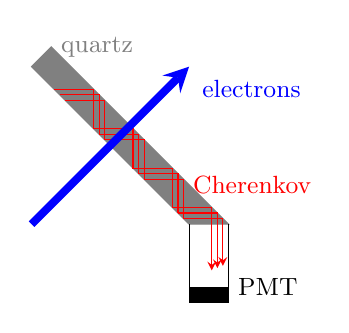
\begin{tikzpicture}[xshift=2cm]
	\draw[fill, Gray] (0, 0) -- ++(-2,2) -- ++(0.25, 0.25) node[right] {\small{quartz}} -- ++(2.25, -2.25) -- (0, 0);
	\draw (0, 0) -- ++(0, -0.8) -- ++(0.5, 0) node[right] {\small{PMT}} -- ++(0, 0.8);
	\draw[fill] (0, -0.8) -- ++(0, -0.2) -- ++(0.5, 0) -- ++(0, 0.2);
	\foreach \i in {1, 2, 3}{
	    \draw[red] (135:\i*0.1) -- ++(0, 0.5) -- ++(-0.5, 0) 
		-- ++(0, 0.5) -- ++(-0.5, 0)
		-- ++(0, 0.5) -- ++(-0.5, 0);
	    \draw[red, -stealth] (135:\i*0.1) -- ++(0.5, 0) -- ++(0, -0.5-\i*0.1);
	    }
	\draw[-stealth,Blue, line width=1mm] (-2, 0) -- ++(2, 2) node[below right] {\small{electrons}};
	\node[red] at (0.8, 0.5) {\small{Cherenkov}};
    \end{tikzpicture}
    \caption[quartz]{Left: CAD drawing of the quartz detector; 
    Middle: schematic plot of the Cherenkov radiation, the angle between 
    the electron and the Cherenkov radiation is 
    $\cos\theta = \frac{v_c}{v_e} = \frac{c}{nv_e} = \frac{1}{n\beta} \approx \frac{1}{n}$;
    Right: electron flux goes through a quartz detector.
    }
    \label{fig:quartz}
\end{figure}

\begin{figure}[!h]
    \centering
    \includegraphics[width=0.7\linewidth]{quartz_QE}
    \caption[photo-electron spectrum of quartz]
    {Simulation result of the photo-electron (PE) spectrum for single electron
    passing through the main detectors. The wider tail in the downstream
    detector is due to particle showering in the upstream quartz \cite{Devi2021}. 
    }
\end{figure}
The width of the photon-electron distribution will increase the statistical uncertainty:
\begin{equation}
    \sigma_{\CA} = \sigma_{\text{stat}} \times \sqrt{1 + \left( \frac{\sigma_{\text{PE}}}{\langle \text{PE} \rangle }\right)^2}
\end{equation}
where $\sigma_{\text{PE}}$ is the RMS of the distribution. The RMS can be parameterized
into two parts: the Gaussian principle part which is inversely proportional to
the quartz thickness and a Landau tail which comes from the showering process
and is proportional the thickness. A thicker thickness enhance the 
photon-electron yield while a thinner one can reduce the showering effect.
The final decision of a 5~mm thickness is a compromise between these two factors 
to minimize the detector resolution $\sigma_{PE}/\langle PE \rangle$. 

\begin{figure}[!h]
    \centering
    \includegraphics[width=\linewidth]{quartz_projection}
    \caption[Electron position distribution, projected on the quartz plane.]
    {Electron position distribution, projected on the quartz plane. 
    The positions of the first four excited states are shown in the left plot. 
    The red rectangle on the right plot shows the relative position of the quartz.
    Plots from Devi Adhikari \cite{Devi2021}.}
\end{figure}

There is a custom motion control system in each arm to move the main detectors.
The control system can be operated remotely, providing the convenience of easily adjusting the position of the main detectors whenever there are changes in the beam conditions or any other aspects of the experimental setup.
% changed gain of the main detectors under a different beam current.

% Can we use it as a calorimeter? How to measure the beam energy?

%%%%%%%%%%%%%%%%%%%%%%%%
\subsubsection{AT Monitors}
% last page of https://prex.jlab.org/DocDB/0000/000096/002/riordan_prex_soft.pdf
About 1~m downstream the main detector is a pair of AT monitors, as shown 
in Fig.~\ref{fig:detectors}, which use exactly the same quartz piece as the 
main detectors. They are used to monitor transverse polarization in the beam.
\begin{figure}[!h]
    % FIXME: source of these 2 plots
    \centering
    \begin{tikzpicture}
	\begin{scope}
	    \node[anchor=south west, inner sep=0] (image) at (0, 0)
	    { 
		\includegraphics[width=0.48\linewidth]{ATL1}
		\includegraphics[width=0.48\linewidth]{ATL2}
	    };
	    \begin{scope}[x={(image.south east)}, y={(image.north west)}]
		\draw[thick, red] (0.06, 0.58) rectangle ++(0.2, 0.11);
		\draw[thick, red] (0.15, 0.35) rectangle ++(0.2, 0.11);
		\node[thick, red] at (0.3, 0.4) {\large \textbf{L-AT1}};
		\draw[thick, blue] (0.568, 0.58) rectangle ++(0.2, 0.11);
		\draw[thick, blue] (0.658, 0.35) rectangle ++(0.2, 0.11);
		\node[thick, blue] at (0.62, 0.63) {\large \textbf{L-AT2}};
	    \end{scope}
	\end{scope}
    \end{tikzpicture}
    \caption[Scatter plot of electrons on the left arm AT monitor plane.]
    {Scatter plot of electrons on the left arm AT monitor plane. 
    Red and blue dots represent electrons scattered either above or below the
    horizontal scattering plane, respectively. The red and blue rectangles
    show the relative positions of the two AT detectors. 
    % So the two AT detectors, are sensitive events of opposite 
    }
\end{figure}

%%%%%%%%%%%%%%%%%%%%%%%%%%%%%%%%%%%%%%%%%%%%%%%%
\subsection{Data AcQuisition (DAQ)}
JLab has its own framework of hardwares and softwares for data acquisition, known
as CODA (CEBAF Online Data Acquisition) \cite{CODA}. CODA is a distributed
system that can be scaled from a few detector channels to tens of thousands of
channels needed in an experiment. CODA version 2.6.2 is used for PREX-II and CREX.
% CODA data structure: https://hallaweb.jlab.org/equipment/daq/dstruct.html

Data acquisition operates in 2 modes: the integrating mode and the counting mode,
both have their own DAQs, because they have different triggers and read from
different detectors.

%%%%%%%%%%%%%%%%%%%%%%%%
\subsubsection{Integrating DAQ}
The integrating DAQ consists of four primary DAQ systems distributed acrosss the injector,
Counting House (CH) and the hall (LHRS/RHRS). They are controlled by the
CODA Run Control system in the CH, and triggered by the helicity signal.

The helicity signal is generated by a helicity control board \cite{Hboard}, which 
is an advanced programmable logic generator, located in the Injector Service Building.
It offers four timing modes: three fixed-frequencies of 30, 120 and 240~Hz
as well as a fourth free-running mode. In the fixed-frequency mode, as used for PREX-II/CREX,
the phase is locked to the `beam sync', which refers to the 60 Hz AC line signal of the accelerator acting as a global timing reference. Consequently, the duration of the last helicity window in a helicity pattern may vary from the others due to the intermittent wandering of the 60 Hz line signal, as depicted as beam sync jitter in the second timing diagram in Fig.~\ref{fig:timing}.

To ensure that all helicity windows have the same integrating time, 
an artificial deadtime is introduce, which is $T_{\text{dead}} = 51.33\ \mu$s,
as shown in Fig.~\ref{fig:integrating_timing}.
This slightly reduces the integration time: $T_{\text{int}} = T_{\text{stable}} - T_{\text{dead}}$.
% Beam sync signal: SCAM module, https://prex.jlab.org/wiki/index.php/Helicity_Control

\begin{figure}
    \centering
    \includegraphics[width=0.9\linewidth]{timing}
    \caption[Helicity timing diagram]
    {Helicity timing diagram. The Tsettle signal (falling edge) marks the  
    beginning of a new helicity window and serve as the reference point (t=0)
    for all timing diagrams. It is transmitted to the CH/hall.
    The QRT (Pattern Sync) signal indicates the start of each helicity pattern,
    it goes to the CH. 
    The Pair Sync signal toggles between 0 and 1, signifying the start and end
    of a helicity pair. It is sent to the CH. This signal is not important, all it
    tells can be inferred from the QRT signal.
    The Hel+ signal decides the helicity of the current window, it goes to the 
    laser table in the injector.
    The Hel- signal acts as the complementary signal to Hel+, so that the board always 
    keeps the same current regardless of the helicity state, preventing helicity 
    correlated electrical pickup from the board. This signal is not shown in the
    plot, it goes to the helicity magnets (the double wien filters).
    The delayed helicity (DLY RPT) signal is delayed by n (specified by the user) 
    windows with respect to the Hel+ signal.
    It tells what the helicity state was n windows before. It goes to the CH. This
    signal is not shown in the plot.}
    \label{fig:timing}
\end{figure}

The helicity signal sent to injector components (PCs, IAs and double Wien filters) 
can be regarded as real-time due to their close proximity. The Tsettle signal, transmitted to Hall A, serves several purposes. When the falling edge of Tsettle is received, it indicates the end of data acquisition in the previous helicity window. It then remains in a hold state for $T_{\text{settle}}$ time to allow for the settling of high voltages in the PCs and the readout of data from the previous helicity window.

The rising edge of Tsettle signifies the start time of data acquisition in the current helicity window. Due to the signal transportation delay in fiber optic cables to Hall A, which is approximately 100~ns, an additional 1~$\mu$s is reserved between Tsettle and the helicity signals to notify Hall A of the helicity change, as depicted in Figure \ref{fig:timing}.

Actually, this 1~$\mu$s delay is not necessary, because $T_{\text{settle}} = 90\ \mu$s is already long 
enough to account for the signal transportation delay in fiber optics cables, as well as the delay 
caused by beam transportation in the accelerator, which is $1.4 \ \text{km/c} = 4.7\ \mu$s.

The actual helicity signal (DLY RPT) sent to Hall A is intentionally delayed 
by 8 helicity windows in PREX-II/CREX. This delay ensures that no monitors 
along the beamline or detectors in the hall know the helicity of the current window, 
making sure that these monitors and detectors are not sensitive to helicity. 

On the DAQ side, we need to verify that observed the helicity pattern aligns 
with expected pattern based on the helicity pattern signal and the 
measured helicity, thus ensuring the accuracy of the helicity information. 

During data analysis, the collected data needs to be shifted by number of 
delayed helicity windows to match the actual helicity pattern. 
The helicity pattern is pseudo-randomly chosen by the helicity board 
using a 30-bit shift register.

% https://prex.jlab.org/DocDB/0001/000187/001/PREX_DAQ_25July18.pdf
The analog signals from the main detectors and various beam monitors are first 
converted to voltage by a customized I-to-V preamplifier developed for the Qweak experiment.
The voltage output is then fed to a 18-bit ADC (Analog-Digital-Converter) for sampling
and integration. This 18-bit ADC was also a product of previous parity experiments. 
The detector signal is sampled every $2\ \mu$s and integrated into four sub-blocks 
within each helicity window. Each sub-block consists of 1024 samples, resulting in
a total of 4096 samples per helicity window at a helicity frequency of 120~Hz.

To ensure proper operation, the ADC is triggered 80~$\mu$s after the start of $T_{\text{settle}}$, as shown in Fig.~\ref{fig:integrating_timing}. This 80~$\mu$s delay allows for a $10\ \mu$s waiting time for 
the ADC to void any possible effects from external triggering Nuclear Instrument Module
(NIM) pulse on the internal signal processing. 

To synchronize the data collection (integration), 
a HAPPEX Timing Board (HAPTB) is used, which receives the Tsettle signal and
produces the integration gate signals, distributing them to each ADC/scalar to trigger
the signal integration/collection.
% HAPTB: https://prex.jlab.org/wiki/index.php/DAQ_Hardware_HAPTB

\begin{figure}
    \centering
    \includegraphics[width=\linewidth]{integrating_timing}
    \caption{Integrating timing}
    \label{fig:integrating_timing}
\end{figure}

Each DAQ is housed in its own VME crate, which contains all the necessary hardware 
modules. A read out controller (ROC) controls the VME crate. All these crates (ROCs) are
managed by a trigger supervisor (TS), which has its own VME crate. The TS is
triggered by the Tsettle signal, and in turn, it triggers the ROCs.
When triggered, each ROC reads the data stored in their memory buffer 
and send it to the CODA system, which will build, transport and store events. 
An analyzer called JAPAN (Just Another Parity ANalyzer) will monitor the 
quality of data in real-time. Additionally, JAPAN can also be used for offline
data analysis.

% \begin{figure}
%     \centering
%     \includegraphics[width=0.5\linewidth]{Coda}
% \end{figure}

%%%%%%%%%%%%%%%%%%%%%%%%
\subsubsection{Counting DAQ}
The two counting DAQs, one for each HRS, differ from the integrating DAQs,
in terms of hardwares and softwares. In contrast to integrating electrons,
the counting DAQ are specifically designed for recording and reconstructing tracks 
of scattered electrons on an indivial basis.

The counting DAQ reads data from the scintillators, VDCs and GEMs, and the main detectors.
It is triggered by the scintillators, different logical combinations of the scintillator
signals could trigger varying counting rates. Most of the time, we used the S0
trigger signal, as discussed in the scintillator sector.

The analyser used for decoding counting mode data is the general Hall A analyser.
This analyzer reads the hit information from each detector and utilizes this information
to reconstruct the trajectory of the scattered electron. By reversing the optics matrix, it can
calculate the electron information such as position, angle and energy at the target. These
information enables the measurements of the scattering angle and $Q^2$, 
aiding in the fine-tune of the optics matrix, detector alignment and background verification.

%%%%%%%%%%%%%%%%%%%%%%%%
\subsubsection{EPICS}
In addition to the two DAQ systems, there is a site-wise slow (relative to the helicity frequency) 
control system, called Experimental Physics and Industrial Control System (EPICS) \cite{EPICS}.
EPICS monitors and controls various important components and parameters throughout
the experimental setup. This includes magnets, beam current/position/energy, 
vacuum level, temperature, gas flow, high voltage supply etc. EPICS polls a series of 
input/output controllers (IOCs) and record their average values about every second.
It allows for real-time monitoring of the entire system: both the accelerator and detectors. 
It provides continuous monitoring and enables the operators to trace the status of the system, facilitating troubleshooting and problem resolution whenever issues arise.
